% PTE Core 模考 43B —— 总整理卷（听·读·说(DI) 合订，自包含；本套未收录写作）
% 编译: xelatex 本文件.tex（跑两遍，目录页码才对）；依赖同目录 img/。
\documentclass[11pt]{article}

% --------- 样式（原 ptestyle.sty，已内联）---------
% ============================================================
%  ptestyle.sty  —  PTE 模考错题整理卷 共享样式
%  编译引擎: XeLaTeX  (中英混排, 需要 Noto CJK 字体)
% ============================================================

\usepackage[a4paper,margin=2cm,headsep=4mm]{geometry}
\usepackage{fontspec}
\usepackage{xeCJK}
\usepackage[table]{xcolor}
\usepackage[normalem]{ulem}        % \sout 删除线
\usepackage{tabularx}
\usepackage{array}
\usepackage{ragged2e}
\usepackage{enumitem}
\usepackage[most]{tcolorbox}
\usepackage{fancyhdr}
\usepackage{graphicx}
\usepackage{pifont}                % \ding{51}=✓ \ding{55}=✗（阅读对错标注）
\usepackage{needspace}
\usepackage{tikz}

% ---------- 字体 ----------
\setmainfont{TeX Gyre Heros}            % 拉丁: Helvetica 风格(纤细清晰)
\setCJKmainfont{Noto Sans CJK SC}
\setCJKsansfont{Noto Sans CJK SC}
\newfontfamily\cjkserif{Noto Serif CJK SC}
\linespread{1.18}
\setlength{\parindent}{0pt}
\setlength{\parskip}{4pt}

% ---------- 配色 ----------
\definecolor{cWrong}{HTML}{D32F2F}     % 红  = 修改 / 错误
\definecolor{cFix}{HTML}{1B7F3B}       % 绿  = 正确建议
\definecolor{cDelete}{HTML}{1565C0}    % 蓝  = 删除
\definecolor{cInsert}{HTML}{7B1FA2}    % 紫  = 插入
\definecolor{cPartial}{HTML}{E07B00}   % 橙  = 部分得分
\definecolor{cNote}{HTML}{0277BD}      % 蓝  = 注解
\definecolor{cAccent}{HTML}{16A085}    % 主题青绿(平台主色)
\definecolor{cWrongBg}{HTML}{FBE0E0}
\definecolor{cDelBg}{HTML}{DCE8FB}
\definecolor{cInsBg}{HTML}{EEE0F5}
\definecolor{cHead}{HTML}{20303A}
\definecolor{cGrayBox}{HTML}{F4F6F7}
\definecolor{cModelBg}{HTML}{EAF7EF}
\definecolor{cYouBg}{HTML}{FFF7F5}
\definecolor{cNoteBg}{HTML}{EAF3FA}
\definecolor{cRule}{HTML}{D7DEE2}

% ---------- 行内批改宏 (复刻平台标注) ----------
% \fix{原词}{正确}  红色删除线 + 绿色上标改正  (修改/拼写/空格)
\newcommand{\fix}[2]{%
  \colorbox{cWrongBg}{\textcolor{cWrong}{\sout{#1}}}%
  \,\textsuperscript{\textcolor{cFix}{\footnotesize #2}}}
% \del{原词}  蓝色删除线  (应删除)
\newcommand{\del}[1]{%
  \colorbox{cDelBg}{\textcolor{cDelete}{\sout{#1}}}%
  \,\textsuperscript{\textcolor{cDelete}{\footnotesize 删}}}
% \ins{词}  紫色下划线  (应插入)
\newcommand{\ins}[1]{%
  \textsuperscript{\textcolor{cInsert}{\footnotesize $\wedge$}}%
  \colorbox{cInsBg}{\textcolor{cInsert}{#1}}}
% \miss{词}  灰色删除线  (口语漏读 / 未作答)
\newcommand{\miss}[1]{\textcolor{gray}{\sout{#1}}}
% \add{原词}{改正}  橙色波浪线 + "补"标签  (平台漏标、本卷补标的错误)
\definecolor{cAdd}{HTML}{E65100}
\newcommand{\add}[2]{%
  \textcolor{cAdd}{\uwave{#1}}%
  \,\textsuperscript{\textcolor{cAdd}{\footnotesize 补：#2}}}
% 高亮(口语发音): 好/中/差
\newcommand{\spk}[2]{\textcolor{#1}{#2}}

% ---------- 评分单元格着色 ----------
\newcommand{\sfull}[1]{\textcolor{cFix}{\bfseries #1}}     % 满分
\newcommand{\spart}[1]{\textcolor{cPartial}{\bfseries #1}} % 部分
\newcommand{\szero}[1]{\textcolor{cWrong}{\bfseries #1}}   % 零/低分

% ---------- 分数小标签 ----------
\newtcbox{\chip}[1][cAccent]{on line, boxsep=2pt, left=4pt, right=4pt, top=1pt,
  bottom=1pt, arc=3pt, colback=#1, colframe=#1, coltext=white, nobeforeafter,
  fontupper=\bfseries\footnotesize}

% ---------- 题块小标题 ----------
\newcommand{\ptesub}[1]{%
  \par\needspace{2\baselineskip}\smallskip
  {\color{cAccent}\rule[-0.2ex]{3pt}{1.05em}}\hspace{6pt}%
  {\bfseries\color{cHead}#1}\par\nopagebreak\smallskip}

% ---------- 题块外框 ----------
% \begin{qblock}{标号·题型}{右上信息(得分/用时)} ... \end{qblock}
\newtcolorbox{qblock}[2]{
  breakable, enhanced, arc=2.5pt,
  colback=white, colframe=cRule, boxrule=0.6pt,
  left=11pt, right=11pt, top=8pt, bottom=10pt,
  toptitle=3pt, bottomtitle=3pt, lefttitle=11pt, righttitle=11pt,
  colbacktitle=cHead, coltitle=white, fonttitle=\bfseries,
  title={#1\hfill\normalfont\bfseries\small #2}}

% ---------- 文本块: 题干 / 范文 / 你的作答 / 建议 ----------
\newtcolorbox{promptbox}{enhanced, breakable, colback=cGrayBox, colframe=cGrayBox,
  arc=2pt, left=8pt, right=8pt, top=6pt, bottom=6pt, boxrule=0pt}
\newtcolorbox{modelbox}{enhanced, breakable, colback=cModelBg, colframe=cModelBg,
  borderline west={3pt}{0pt}{cFix}, arc=1pt, left=8pt, right=8pt, top=6pt, bottom=6pt, boxrule=0pt}
\newtcolorbox{youbox}{enhanced, breakable, colback=cYouBg, colframe=cYouBg,
  borderline west={3pt}{0pt}{cWrong}, arc=1pt, left=8pt, right=8pt, top=6pt, bottom=6pt, boxrule=0pt}
\newtcolorbox{notebox}{enhanced, breakable, colback=cNoteBg, colframe=cNoteBg,
  borderline west={3pt}{0pt}{cNote}, arc=1pt, left=8pt, right=8pt, top=6pt, bottom=6pt, boxrule=0pt}

% ---------- 评分表 ----------
% 用法见正文; 这里给表头宏
\newcommand{\scorehead}{%
  \rowcolors{2}{cGrayBox}{white}
  \arrayrulecolor{cRule}}

% ---------- 章节大标题 ----------
\newcommand{\ptesection}[3]{% #1=中文名 #2=英文名 #3=该项分数
  \addcontentsline{toc}{section}{#1}%
  \needspace{6\baselineskip}
  \begin{tcolorbox}[enhanced, colback=cAccent, colframe=cAccent, sharp corners,
     left=14pt, right=14pt, top=10pt, bottom=10pt, boxrule=0pt]
    {\fontsize{20}{24}\selectfont\bfseries\color{white} #1\ \ }%
    {\large\color{white!85} #2}\hfill
    {\large\color{white}本项得分\ \ }{\fontsize{22}{24}\selectfont\bfseries\color{white} #3}%
    \ {\color{white!85}/ 90}
  \end{tcolorbox}}

% ---------- 题型小节分隔 (口语 RA/RS/DI/RTS/ASQ 等) ----------
\newcommand{\ptetask}[2]{%
  \addcontentsline{toc}{subsection}{#1\ #2}%
  \needspace{4\baselineskip}\medskip
  \begin{tcolorbox}[enhanced, colback=cHead, colframe=cHead, sharp corners,
     left=12pt, right=12pt, top=5pt, bottom=5pt, boxrule=0pt]
    {\large\bfseries\color{white} #1}\ \ {\color{white!80} #2}
  \end{tcolorbox}\smallskip}

% ---------- 口语 AI 语音识别着色 (复刻平台: 优/良/差 + 停顿) ----------
\definecolor{cSpkGood}{HTML}{2E9E5B}   % 优 绿
\definecolor{cSpkOk}{HTML}{C77F00}     % 良 黄/琥珀
\definecolor{cSpkBad}{HTML}{E0352B}    % 差 红
\newcommand{\sg}[1]{\textcolor{cSpkGood}{#1}}   % 优
\newcommand{\sy}[1]{\textcolor{cSpkOk}{#1}}     % 良
\newcommand{\sr}[1]{\textcolor{cSpkBad}{#1}}    % 差
\newcommand{\smiss}[1]{\textcolor{cSpkBad}{\sout{#1}}}  % 漏读 (红删除线)
\newcommand{\pse}{{\color{gray}\,/\,}}          % 停顿
\newcommand{\asrlegend}{{\footnotesize\color{gray}AI 语音识别\quad
  {\color{cSpkGood}\textbullet}\,优\ \ {\color{cSpkOk}\textbullet}\,良\ \
  {\color{cSpkBad}\textbullet}\,差\ \ {\color{gray}/}\,停顿\ \
  {\color{cSpkBad}\sout{词}}\,漏读}}
\newtcolorbox{asrbox}{enhanced, breakable, colback=white, colframe=cRule,
  boxrule=0.6pt, arc=1pt, left=8pt, right=8pt, top=6pt, bottom=6pt}

% ---------- 中文翻译行 ----------
\newcommand{\zh}[1]{{\footnotesize\textcolor{cNote}{\textbf{译}}\ \textcolor{gray}{#1}}}

% ---------- 阅读填空 / 选择 对错标注 ----------
\newcommand{\rok}[1]{{\color{cFix}\ding{51}\,#1}}                 % 选对(绿勾 + 词)
\newcommand{\rno}[2]{{\color{cWrong}\ding{55}\,\sout{#1}}\,{\footnotesize\color{cFix}(答案:\,#2)}}  % 选错: 你的(红删) + (答案:正确)
\newcommand{\rblank}[1]{{\color{cFix}\underline{\,#1\,}}}         % 直接给空的正确答案(无你的作答时)

% ---------- 听力专用 ----------
\newcommand{\hiw}[2]{{\color{cWrong}\uline{#1}}\,{\footnotesize\color{cFix}(听:#2)}} % HIW: 屏幕错词(红下划线)+ 实际读音
\newcommand{\lhit}[1]{{\color{cFix}#1}}                           % WFD: 命中的词(绿)
\newcommand{\lmiss}[1]{{\color{cWrong}\sout{#1}}}                 % WFD: 多余/错误的词(红删, 1B 配色)
% ---- WFD 逐词批改 · 本套 2B 平台配色（与 1B 相反）：绿=命中 / 红括号=漏写 / 灰删除线=多写或听错 ----
% 说明: 2B 平台把"漏写"标红(加括号)、"多写/听错"标灰删除线; 本卷忠于原图按此复刻。
\newcommand{\womit}[1]{{\color{cWrong}(#1)}}                      % WFD: 漏写(正确答案有、你没写)——红色括号
\newcommand{\wbad}[1]{{\color{gray}\sout{#1}}}                    % WFD: 多写/听错(你写了但错)——灰删除线
\newcommand{\wfdlegend}{{\footnotesize\color{gray}WFD 配色：\
  {\color{cFix}命中}\ \ {\color{cWrong}(漏写)}\ \ {\color{gray}\sout{多写/听错}}}}

% ---------- 颜色图例 ----------
\newcommand{\ptelegend}{%
  \begin{tcolorbox}[enhanced, colback=cGrayBox, colframe=cRule, boxrule=0.5pt,
    arc=2pt, left=10pt, right=10pt, top=6pt, bottom=6pt]
  {\bfseries\color{cHead}颜色说明\quad}
  \fix{改}{正}~修改/拼写\quad
  \del{删}~应删除\quad
  \ins{插}~应插入\quad
  \add{补}{改正}~平台漏标(本卷补标)\quad
  {\color{cFix}\rule{1em}{0.6em}}~范文/正确\quad
  {\color{cNote}\rule{1em}{0.6em}}~AI 建议
  \end{tcolorbox}}

% ---------- 页眉页脚 ----------
\pagestyle{fancy}
\fancyhf{}
\renewcommand{\headrulewidth}{0.4pt}
\renewcommand{\footrulewidth}{0pt}
\fancyhead[L]{\footnotesize\color{cHead}\bfseries PTE Core 模考 43B}
\fancyhead[R]{\footnotesize\color{gray} 错题与详解整理卷}
\fancyfoot[C]{\footnotesize\color{gray}\thepage}
\renewcommand{\contentsname}{目录\quad Contents}

\begin{document}

% --------- 封面（原 cover.tex）---------
% ---------- 封面 / 成绩总览 ----------
\definecolor{mListen}{HTML}{1F3A5F}
\definecolor{mRead}{HTML}{C2D70B}
\definecolor{mSpeak}{HTML}{4D4D4D}
\definecolor{mWrite}{HTML}{A01B7D}

\begin{titlepage}
\thispagestyle{empty}
\centering
\vspace*{1.4cm}

{\fontsize{30}{36}\selectfont\bfseries\color{cHead} PTE Core 模考 43B}\\[4mm]
{\fontsize{17}{20}\selectfont\color{cAccent}\bfseries 错题与详解 · 整理卷}\\[3mm]
{\color{gray} APEUni / 猩际 完整模考 43B（8.7 新考试版本）　·　提交时间 2026-07-03 17:45}\\[1.2cm]

% ---- 总分 ----
\begin{tcolorbox}[width=0.62\textwidth, halign=center, enhanced,
  colback=cAccent, colframe=cAccent, arc=6pt, boxrule=0pt, top=10pt, bottom=10pt]
  {\color{white}\large 总分 Overall}\\[2pt]
  {\fontsize{46}{50}\selectfont\bfseries\color{white} 29}
\end{tcolorbox}

\vspace{1.0cm}

% ---- 四项分数条形图（条长 = 得分 / 90，比例 1pt = 1/9 cm）----
\begin{tcolorbox}[width=0.84\textwidth, enhanced, colback=white, colframe=cRule,
  boxrule=0.8pt, arc=4pt, left=18pt, right=18pt, top=14pt, bottom=14pt]
\setlength{\tabcolsep}{6pt}\renewcommand{\arraystretch}{1.7}
\sffamily
\begin{tabular}{@{}r@{\hskip 8pt}l@{\hskip 10pt}l@{}}
 \bfseries Listening 听力 & {\color{mListen}\rule{3.56cm}{0.42cm}} & {\bfseries\large 32}\\
 \bfseries Reading 阅读   & {\color{mRead}\rule{5.67cm}{0.42cm}}   & {\bfseries\large 51}\\
 \bfseries Speaking 口语  & {\color{mSpeak}\rule{1.33cm}{0.42cm}}  & {\bfseries\large 12}\\
 \bfseries Writing 写作   & {\color{mWrite}\rule{2.33cm}{0.42cm}}  & {\bfseries\large 21}\\
\end{tabular}\\[2mm]
{\footnotesize\color{gray} 满分 90　|　刻度: 条长 = 得分 / 90}
\end{tcolorbox}

\vspace{0.8cm}

% ---- 本卷收录范围 ----
\begin{tcolorbox}[width=0.84\textwidth, enhanced, colback=cModelBg, colframe=cFix,
  boxrule=0pt, borderline west={3pt}{0pt}{cFix}, arc=3pt, left=14pt, right=14pt, top=8pt, bottom=8pt]
{\bfseries\color{cHead}本卷收录}\quad{\small 本次只做了\textbf{阅读}与\textbf{听力}，另收录口语的 \textbf{DI 看图说话}题；
共 \textbf{阅读 15 题 · 听力 15 题 · 口语 DI 5 题}。写作及口语其它题型（RA/RS/RTS/ASQ 等）未收录。}
\end{tcolorbox}

\vfill
\begin{flushleft}\small\color{gray}
\textbf{说明:}本卷由本次模考的题目与"答案 \& 解析"截图逐题誊写、重新排版而成,完整保留每道题的
\emph{题干 / 原文、选项 / 词库、你的作答、正确答案、平台中文解析与逐项得分}。\\
所有对错按平台标注用颜色标出(\rok{绿勾}=选对; {\color{cWrong}\ding{55}}\,红叉=选错并给出正确答案)。原始截图不可复制、仅能看图,本卷内容均为人工对照誊录,若与原图有出入以原图为准。
\emph{个别题(阅读 R01 选项 3--5、R14 选项 A)在原图中被平台悬浮条遮挡,已照实标注。}
\end{flushleft}
\vspace{4mm}
\ptelegend
\end{titlepage}

% --------- 目录 + 本卷概览 ---------
\clearpage
\tableofcontents
\bigskip

{\large\bfseries\color{cAccent}本卷概览}\par\smallskip
{\small
\begin{tabularx}{\linewidth}{@{}l c >{\RaggedRight\arraybackslash}X r@{}}
\rowcolor{cHead}\textcolor{white}{\bfseries 部分} & \textcolor{white}{\bfseries 题量} & \textcolor{white}{\bfseries 题型构成} & \textcolor{white}{\bfseries 本项得分}\\
听力 Listening & 15 & SST · MCM-L\,$\times$2 · FIB-L\,$\times$2 · HCS\,$\times$2 · MCS-L\,$\times$2 · SMW · HIW\,$\times$2 · WFD\,$\times$3 & 32 / 90\\
阅读 Reading & 15 & FIB\,$\times$5 · MCM-R\,$\times$2 · RO\,$\times$2 · FIBD\&D\,$\times$4 · MCS-R\,$\times$2 & 51 / 90\\
口语 Speaking（仅 DI）& \phantom{0}5 & DI\,$\times$5（RA/RS/RTS/ASQ 等题型未收录）& 12 / 90\phantom{$^*$}\\
\end{tabularx}}
\par\smallskip
{\footnotesize\color{gray}本次模考总分 29（听力 32 / 阅读 51 / 口语 12 / 写作 21，写作未收录本卷）。口语一栏
12/90 为该考生口语部分\emph{官方总分}（含未收录的 RA/RS/RTS/ASQ 等题型），非本卷 5 道 DI 的得分总和。
颜色与标注沿用各部分；本合订本顺序为「听·读·说（DI）」。}

\clearpage
% --------- 已收录部分正文 ---------
% ===== sec_listening_body.tex =====
% ===================== 听力 Listening =====================
\ptesection{听力}{Listening · SST + MCM-L + FIB-L + HCS + MCS-L + SMW + HIW + WFD}{32}

\vspace{1mm}
{\small\color{gray} 本部分共 \textbf{15 题}：\textbf{SST 概述口语}Q1、\textbf{MCM-L 多选}Q2--3、\textbf{FIB-L 听力填空（打字）}Q4--5、\textbf{HCS 选最佳概括段}Q6--7、\textbf{MCS-L 单选}Q8--9、\textbf{SMW 选词}Q10、\textbf{HIW 找错词}Q11--12、\textbf{WFD 听写句子}Q13--15。每题保留\textbf{录音原文/文字稿}（MCM-L/HCS/MCS-L/SMW/HIW 均附全文字稿）、你的作答与平台评分，并附\textbf{中文翻译}。
标注约定：FIB-L 空处 \rok{绿勾}=对、{\color{cWrong}\ding{55}}\,红叉=错并给答案；HIW 屏幕错词用{\color{cWrong}\uline{红下划线}}标出并括注\,{\footnotesize\color{cFix}(听:实际读音)}；WFD 逐词批改本套配色为 \wfdlegend 。
本套听力官方得分 \textbf{32 / 90}。}
\vspace{1mm}

{\small\color{gray}\textbf{说明：}Q1 SST 录音原文文字稿由平台「查看原题」补录；其余题型的录音文字稿复盘页均直接给出，已照抄。}
\vspace{2mm}

\newcolumntype{Z}{>{\RaggedRight\arraybackslash}X}

% ---------------- Q1 ----------------
\begin{qblock}{Q1\quad SST \#712\ \ Environmental Conservation}{概述口语 · 评分 \textcolor{cAccent}{\bfseries 7.2 / 12}}
\ptesub{录音原文 Transcript}
\begin{promptbox}
Now let us delve into the critical importance of environmental conservation and the urgent need to protect our planet.

Our environment is the foundation of life on Earth. It provides us with clean air, fresh water, and fertile soil, all essential for our survival. When we neglect environmental conservation, we jeopardize these vital resources.

Furthermore, a healthy environment is key to biodiversity. Ecosystems thrive when they are in balance, and the diversity of species sustains the overall health of the planet. Conservation efforts help protect endangered species and maintain ecological equilibrium.

Moreover, environmental conservation is closely linked to our quality of life. Pollution, deforestation, and climate change have far-reaching consequences, including adverse effects on public health and economic stability. Investing in conservation is an investment in our well-being and future prosperity.

In conclusion, environmental conservation is not just an ethical responsibility; it is a fundamental necessity. By safeguarding our environment, we ensure a sustainable future for ourselves and future generations, preserving the beauty and richness of our planet.
\end{promptbox}
\zh{现在让我们深入探讨环境保护的至关重要性，以及保护地球的迫切需要。我们的环境是地球生命的根基，它为我们提供了清洁的空气、新鲜的水源和肥沃的土壤，这些都是我们生存所必需的。当我们忽视环境保护时，我们就是在危及这些至关重要的资源。此外，健康的环境是生物多样性的关键：生态系统在平衡状态下才能繁荣发展，物种的多样性维系着地球的整体健康；保护工作有助于保护濒危物种、维持生态平衡。而且，环境保护与我们的生活质量息息相关：污染、森林砍伐和气候变化会带来深远的后果，包括对公共健康和经济稳定的不利影响；投资于环保就是投资于我们的福祉与未来的繁荣。总之，环境保护不仅是一种道德责任，更是一种根本必要；通过保护环境，我们为自己和后代确保可持续的未来，留存地球的美丽与富饶。}
\ptesub{你的概述 Your Summary}
\begin{youbox}
The \fix{reprot}{report} mainly mentioned \fix{about environment}{environmental} conservation and the clean air on the earth. It also mentioned that \fix{the environment}{environmental} conservation means the quality of life and the economy of \del{the} society. And it also mentioned the responsibility and the sustainable development of the planet. Overall, it mentioned the importance of \fix{the environment}{environmental} conservation.
\end{youbox}
\zh{这篇报告主要提到了环境保护和地球清洁空气的问题。它还提到，环境保护意味着生活质量和社会经济。此外，它还提到了责任以及地球的可持续发展。总的来说，它提到了环境保护的重要性。}
{\footnotesize\color{gray}（平台彩色标注：reprot —— 拼写错误，应为 report；about environment / the environment（两处）—— 均应改为形容词 environmental；economy of the society 中 the 建议删除。）}
\ptesub{AI 评分明细（满分 12）}
\begin{notebox}
{\renewcommand{\arraystretch}{1.35}
\begin{tabularx}{\linewidth}{@{}l c Z@{}}
\textbf{单项} & \textbf{得分} & \textbf{AI 建议}\\[2pt]
Content（内容）& \spart{3.2 / 4} & 内容很棒。\\
Form（形式）& \sfull{2 / 2} & Form 很棒，这是必拿分数。\\
Grammar（语法）& \szero{0 / 2} & 语法在 SST 中占分比很重，但其实又非常容易提高。丢分这么严重，有点不应该哦。建议找老师咨询下迅速提高的技巧。\\
Spelling（拼写）& \spart{1 / 2} & 拼写错 1 个就单词扣 1 分，2 个就会扣 2 分，丢分很可惜哦。\\
Vocabulary（词汇）& \spart{1 / 2} & PTE 对词汇不要求很难，但需要恰当。\\
\end{tabularx}}
\smallskip
\textbf{本题分值}\ 12 分\qquad\textbf{你的总得分}\ \textcolor{cAccent}{\bfseries 7.2 / 12}\qquad{\footnotesize\color{gray}评分标准 PTEA SST V2.0}
\end{notebox}
\smallskip
{\footnotesize\color{gray}（答题用时 10:00；AI 提升建议：回答的关键内容点不足。）}
\end{qblock}

% ---------------- Q2 ----------------
\begin{qblock}{Q2\quad MCM-L \#102\ \ Time Famine}{多选 · 评分 \textcolor{cAccent}{\bfseries 0 / 2}}
\ptesub{录音原文 Transcript}
\begin{promptbox}
A team of researchers finds that shelling out for services that save time can bring greater feelings of life satisfaction than, say, simply buying more stuff. The results appear in the Proceedings of the National Academy of Sciences.

It's safe to say that most of us regularly feel crunched for time. So much so that we are experiencing what Ashley Whillans of the Harvard Business School, the lead author of the study, describes as a ``time famine.'' And like any famine, this chronic lack of time takes its toll on our health.

``When we feel like our to-do lists are longer than the hours that we have time in the day to complete them, we can feel as if our life is spiraling out of control, thereby undermining our personal well-being.''

Well, if time is money, Whillans and her team wondered whether money that's used to buy time could offer some relief. Like paying someone else to clean the house, mow the lawn, or deliver the groceries.
\end{promptbox}
\zh{一组研究人员发现，花钱购买节省时间的服务比单纯多买东西更能带来生活满意度，该结果发表于《美国国家科学院院刊》。可以肯定地说，我们大多数人都经常感到时间紧迫，以至于我们正在经历哈佛商学院、该研究主要作者 Ashley Whillans 所描述的"时间饥荒"。和任何饥荒一样，这种长期缺乏时间会损害我们的健康。"当我们觉得待办事项清单比一天里能用来完成它们的时间还长时，我们会感觉生活正在失控，从而损害我们的个人幸福感。"如果说时间就是金钱，Whillans 和她的团队想知道，用来买时间的钱是否能带来一些缓解——比如付钱请人打扫房子、割草坪或者送杂货。}
\ptesub{题目 Question}
\begin{notebox}According to the speaker, which services are the time-saving services?\end{notebox}
\ptesub{选项 Choices（正确项绿色加粗）}
{\small
A) Purchasing more supplies and goods.\\
{\color{cFix}\textbf{B) Hiring someone to walk the dog.}}\\
C) Making a to-do list and completing it.\\
{\color{cFix}\textbf{D) Hiring a babysitter to take care of the baby.}}\\
E) Repairing the computer.}
\par\smallskip
\textbf{正确答案}\ \textcolor{cFix}{\bfseries B, D}\qquad\textbf{你的答案}\ {\color{cWrong}\bfseries C}\qquad\textbf{本题得分：}\ {\color{cAccent}\bfseries 0 / 2}\quad{\footnotesize\color{gray}（用时 01:07）}
\end{qblock}

% ---------------- Q3 ----------------
\begin{qblock}{Q3\quad MCM-L \#106\ \ Hair}{多选 · 评分 \textcolor{cAccent}{\bfseries 1 / 2}}
\ptesub{录音原文 Transcript}
\begin{promptbox}
All mammals have hair---commonly called fur when it's on your cat or a koala. And the thickness of individual hairs varies from species to species. For example, elephant hairs are more than four times thicker than a strand from an adult human.

``Normally, when the animal is larger, the hair tends to be thicker.''

University of California, San Diego, materials scientist Wen Yang. She's interested in how biological structures like hair hold up under stress. That interest comes from a desire to design better synthetic materials.

Yang's team tested the tensile strength of hair from eight different mammal species, including humans. They subjected those hairs to increasing levels of tension until the fibers broke. The researchers assumed that thick hair---from giraffes, elephants and boars, for example---would be more robust. But they were wrong.
\end{promptbox}
\zh{所有哺乳动物都有毛发——长在猫或考拉身上时通常叫皮毛。不同物种间单根毛发的粗细各不相同，例如象毛比成年人的一根头发粗四倍多。"通常动物越大，毛发往往越粗。"加州大学圣地亚哥分校材料科学家 Wen Yang 对生物结构（如毛发）如何承受压力很感兴趣，这一兴趣源于想要设计更好的合成材料。Yang 的团队测试了包括人类在内的八种不同哺乳动物毛发的抗拉强度，让这些毛发承受不断增加的张力，直到纤维断裂。研究人员本以为粗毛（例如长颈鹿、大象和野猪的毛）会更结实，但他们错了。}
\ptesub{题目 Question}
\begin{notebox}Which of the following statements about hair are correct?\end{notebox}
\ptesub{选项 Choices（正确项绿色加粗）}
{\small
{\color{cFix}\textbf{A) Generally speaking, the size of an animal is directly proportional to the thickness of its hair.}}\\
B) Cats have thicker hairs than elephants.\\
C) The function of hairs is to protect the body.\\
{\color{cFix}\textbf{D) Different species have different hair thickness.}}\\
E) The thick hairs on giraffes, elephants are stronger than small animals.}
\par\smallskip
\textbf{正确答案}\ \textcolor{cFix}{\bfseries A, D}\qquad\textbf{你的答案}\ \textcolor{cFix}{\bfseries D}\qquad\textbf{本题得分：}\ {\color{cAccent}\bfseries 1 / 2}\quad{\footnotesize\color{gray}（用时 01:05；漏选 A）}
\end{qblock}

% ---------------- Q4 ----------------
\begin{qblock}{Q4\quad FIB-L \#4}{听力填空（打字）· 评分 \textcolor{cAccent}{\bfseries 1 / 4}}
\ptesub{录音原文 Transcript（含填空作答）}
\begin{promptbox}
An important question about education is, then, why do some types of students achieve success easily and others struggle to do well? Well, one theory is that there is a \rno{generic}{genetic} reason for academic achievement. What I mean by that is, a certain innate, measurable level of \rno{intellegent}{intelligence}. Another frequently discussed theory is environmental factors, such as the effect of home and family upbringing. A final reason is related to the teaching and learning \rok{process} within educational institutions, and the way it is organized, administered and \rno{excessed}{assessed}.
\end{promptbox}
\zh{关于教育的一个重要问题是，为什么有些学生轻易就能取得成功，而另一些却难以做好？一种理论认为，学业成就有其遗传方面的原因，也就是说存在一种与生俱来的、可测量的智力水平。另一种常被讨论的理论是环境因素，比如家庭教养的影响。最后一个原因与教育机构内部的教与学过程，以及其组织、管理和评估的方式有关。}
\par\smallskip
\textbf{你的作答：}\ {\color{cWrong}generic, intellegent}, process, {\color{cWrong}excessed}\qquad\textbf{本题得分：}\ {\color{cAccent}\bfseries 1 / 4}\quad{\footnotesize\color{gray}（用时 02:17；仅第 3 空 process 正确，正确为 genetic / intelligence / process / assessed）}
\end{qblock}

% ---------------- Q5 ----------------
\begin{qblock}{Q5\quad FIB-L \#7\ \ Language Learning}{听力填空（打字）· 评分 \textcolor{cAccent}{\bfseries 3 / 5}}
\ptesub{录音原文 Transcript（含填空作答）}
\begin{promptbox}
Learning a language in the classroom is never easy and, quite \rno{fractly}{frankly}, it's not the way that most people would choose to learn if they had other \rno{（未作答）}{options}. Having said that, there are plenty of reasons for keeping languages on the school curriculum. For one thing, a fair number of students go on to take jobs in business and commerce that require a \rok{basic} knowledge of a second language. When you talk to young \rok{employees} in top companies, it seems that they had a career plan from the start: they were motivated to find additional things to put on their CVs --- and of course language is one of those added, but \rok{significant} extras.
\end{promptbox}
\zh{在课堂上学习一门语言从来都不容易，坦率地说，如果人们还有别的选择，这并不是大多数人会选择的学习方式。话虽如此，学校课程仍保留语言课有很多理由。一方面，相当一部分学生日后会从事需要基本第二语言知识的商业岗位。当你和大公司的年轻员工交谈时，似乎他们从一开始就有职业规划：他们有动力去寻找能写进简历的附加项——语言当然就是其中之一，虽是附加项，却也是重要的加分项。}
\par\smallskip
\textbf{你的作答：}\ {\color{cWrong}fractly}, {\color{cWrong}（空）}, basic, employees, significant\qquad\textbf{本题得分：}\ {\color{cAccent}\bfseries 3 / 5}\quad{\footnotesize\color{gray}（用时 01:29；第 1 空 fractly→frankly，第 2 空未作答→options）}
\end{qblock}

% ---------------- Q6 ----------------
\begin{qblock}{Q6\quad HCS \#80\ \ Mental Health}{选择最佳概括段 · 评分 \textcolor{cAccent}{\bfseries 1 / 1}}
\ptesub{录音原文 Transcript}
\begin{promptbox}
One of the great contributing factors to mental illness is the idea that we should at all costs and at all times be well. We suffer far more than we should because of how long it can take many of us until we allow ourselves to fall properly and usefully ill. In a crisis, our chances of getting better rely to a significant extent on having the right relationship to our illness: an attitude which is relatively unfrightened by our distress, which isn't overly in love with the idea of seeming at all times `normal', which can allow us to be deranged for a while in order one day to reach a more authentic kind of sanity. It will help us immensely in this quest if the images of mental illness we can draw on at this time do not narrowly imply that our ailment is merely a freakish and pitiable possibility, if we can appeal to images that tease out the universal and dignified themes of our state, so that we do not --- on top of everything else --- have to fear and hate ourselves for being unwell.
\end{promptbox}
\zh{导致精神疾病的一大因素，是我们认为自己应当不惜一切代价、任何时候都保持健康。我们所承受的痛苦，往往远超本应承受的程度，因为许多人要花很长时间才能允许自己恰当而有益地"生病"。在危机中，我们能否好转，在很大程度上取决于我们与自身疾病之间是否建立了正确的关系：一种不那么害怕自身痛苦的态度，一种不过分执着于时时表现"正常"的态度——这能让我们暂时"癫狂"一阵子，以便有朝一日达到一种更真实的理智状态。如果此时我们所能借助的精神疾病形象，不狭隘地暗示我们的病痛只是一种古怪而可怜的可能性，而是能借助那些揭示出我们境况中普遍而有尊严的主题的形象，那么这将极大地帮助我们完成这一追寻，让我们不至于在其他一切之外，还要因为生病而害怕、憎恨自己。}
\ptesub{题目 Question}
\begin{notebox}Click on the paragraph that best relates to the recording.\end{notebox}
\ptesub{选项 Choices（正确项绿色加粗）}
{\small
A) People are now living under great stress, so we are facing severe mental illness that can cost us a lot. To solve this problem, it is suggested that we have a strong relationship with others, and try our best not to fear or hate ourselves when we are feeling unwell.\\
{\color{cFix}\textbf{B) There is no need that we should feel well all the time: we can feel disappointed or upset sometimes. We need to find the right relationship with our illness so that it does not cause us too much concern. So we don't necessarily fear or hate it when we feel unwell.}}\\
C) A freakish and pitiable possibility is that when we are feeling unwell, we are more likely to get deranged. Then, our mind allows us to be more worried and afraid. How bad this situation is largely depends on whether we can reach a more authentic kind of sanity or not.\\
D) The idea that we should at all costs and at all times be well alleviates our mental illness. Although we can feel deranged occasionally, this is not a normal state. Feeling ill is not proper, useful or dignified, so it implies that we need to rely on a right relationship to deal with it.}
\par\smallskip
\textbf{正确答案}\ \textcolor{cFix}{\bfseries B}\qquad\textbf{你的答案}\ \textcolor{cFix}{\bfseries B}\qquad\textbf{本题得分：}\ {\color{cAccent}\bfseries 1 / 1}\quad{\footnotesize\color{gray}（用时 01:31，正确）}
\end{qblock}

% ---------------- Q7 ----------------
\begin{qblock}{Q7\quad HCS \#81\ \ What Democracy Breeds}{选择最佳概括段 · 评分 \textcolor{cAccent}{\bfseries 0 / 1}}
\ptesub{录音原文 Transcript}
\begin{promptbox}
In a chapter of Democracy in America entitled why the Americans are often so restless in the midst of their prosperity? De Tocqueville sketched an enduring analysis of the relationship between high expectations and dissatisfaction between political equality and envy. He wrote, when all the prerogatives of birth and fortune have been abolished, when every profession is open to everyone, an ambitious man may think it is easy to launch himself on a great career, and feel that he has been called to no common destiny. But this is a delusion which experience quickly corrects. When inequality is the general rule in society the greatest inequalities attract no attention. But when everything is more or less level, the slightest variation is noticed. That is the reason for the strange melancholy often haunting inhabitants of democracies in the midst of abundance, and of that disgust with life sometimes gripping them even in calm and easy circumstances.
\end{promptbox}
\zh{在《论美国的民主》中题为"美国人为何常常在繁荣中焦躁不安"的一章里，托克维尔对高期望与不满、政治平等与嫉妒之间的关系作了历久弥新的分析。他写道，当出身和财富的一切特权都被废除、当人人都能从事任何职业时，一个雄心勃勃的人可能会认为轻而易举就能开创一番伟大事业，觉得自己被赋予了非凡的命运；但这是一种幻觉，经验很快会纠正它。当不平等是社会普遍规则时，最大的不平等也不会引人注意；但当一切大致趋于平等时，最微小的差异都会被察觉。这正是民主国家的居民即便身处富足，也常常被一种奇怪的忧郁困扰，甚至在平静安逸的环境中也会被那种对生活的厌恶所攫住的原因。}
\ptesub{题目 Question}
\begin{notebox}Click on the paragraph that best relates to the recording.\end{notebox}
\ptesub{选项 Choices（正确项绿色加粗）}
{\small
A) To launch oneself on a great career, a person needs to be very ambitious and insightful. Even in the calm and easy circumstance, he or she has to pay attention to even the slightest variation in the market, which changes fast in the modern era.\\
B) What is haunting inhabitants of democracies is dissatisfaction of political inequality. The Americans will not feel melancholy until all the prerogatives of birth and fortune have been abolished. They will feel safer and happier when everything is more or less level.\\
C) In the midst of their prosperity, every profession is open to every American. People do not have to envy each other, and they believe a completely equal society is no more a delusion. But people with higher expectations tend to feel more disappointed with life.\\
{\color{cFix}\textbf{D) By analyzing political equality and envy and expectations and dissatisfaction, De Tocqueville mentioned that when everyone is living in a basically equal environment, even the slightest inequality will be noticed. This is the reason that the Americans are often restless even in a cozy circumstance.}}}
\par\smallskip
\textbf{正确答案}\ \textcolor{cFix}{\bfseries D}\qquad\textbf{你的答案}\ {\color{cWrong}\bfseries A}\qquad\textbf{本题得分：}\ {\color{cAccent}\bfseries 0 / 1}\quad{\footnotesize\color{gray}（用时 01:17）}
\end{qblock}

% ---------------- Q8 ----------------
\begin{qblock}{Q8\quad MCS-L \#123\ \ Parties}{单选 · 评分 \textcolor{cAccent}{\bfseries 1 / 1}}
\ptesub{录音原文 Transcript}
\begin{promptbox}
Since 1852, every US president has been a member of one of the country's two major political parties, the Republican party or the Democratic party. Democrats generally support higher taxes, so they can fund more government programs. Republicans generally prefer lower taxes and smaller government. These two parties tend to reflect relatively moderate political views.

But there are several other smaller parties on the fringes, including the Libertarian, Constitution, Socialist or Green Parties. Or you can just be an independent not affiliated with any party. Third parties are not that big. But they can have a major influence on presidential elections, by taking away votes from the two major party candidates, which in some years can be a deciding factor in the race to become president.
\end{promptbox}
\zh{自 1852 年以来，每一任美国总统都属于该国两大主要政党之一——共和党或民主党。民主党通常支持提高税收，以资助更多政府项目；共和党通常倾向于降低税收、缩小政府规模。这两个政党往往反映相对温和的政治立场。但也有其他一些边缘小党，包括自由意志党、宪法党、社会党或绿党，你也可以做一个不隶属任何政党的独立人士。第三方规模不大，但它们能通过从两大党候选人那里分走选票，对总统选举产生重大影响，在某些年份甚至可能成为决定谁当选总统的关键因素。}
\ptesub{题目 Question}
\begin{notebox}Which statement about the US parties is NOT true?\end{notebox}
\ptesub{选项 Choices（正确项绿色加粗）}
{\small
A) Apart from the Republican party and the Democratic party, there are other parties as well.\\
B) Democrats usually want taxes to increase so as to support more government programs.\\
C) Republicans are unwilling to enlarge the government and often reject higher taxes.\\
{\color{cFix}\textbf{D) Third parties always play a marginal role in the presidential elections in America.}}}
\par\smallskip
\textbf{正确答案}\ \textcolor{cFix}{\bfseries D}\qquad\textbf{你的答案}\ \textcolor{cFix}{\bfseries D}\qquad\textbf{本题得分：}\ {\color{cAccent}\bfseries 1 / 1}\quad{\footnotesize\color{gray}（用时 01:06，正确）}
\end{qblock}

% ---------------- Q9 ----------------
\begin{qblock}{Q9\quad MCS-L \#122\ \ Washington}{单选 · 评分 \textcolor{cAccent}{\bfseries 0 / 1}}
\ptesub{录音原文 Transcript}
\begin{promptbox}
Washington is a monumental city, a showcase capital with iconic views. And that's because most planned public projects go through the Commission of Fine Arts, a presidentially appointed panel established by Congress in 1910. The idea was to really lift the image of the city as an important international capital, and to really push that idea of dignity and beauty and all these things that you know really contribute to the image of the city.
\end{promptbox}
\zh{华盛顿是一座宏伟的城市，是一个拥有标志性景观的门面首都。这是因为大多数规划中的公共项目都要经过美术委员会审核——这是一个由国会于 1910 年设立、由总统任命成员的专门小组。其设想是真正提升这座城市作为重要国际首都的形象，真正推动那种庄重与美感的理念，以及所有这些真正有助于城市形象的事物。}
\ptesub{题目 Question}
\begin{notebox}For what purpose was the Commission of Fine Arts established in the first place?\end{notebox}
\ptesub{选项 Choices（正确项绿色加粗）}
{\small
{\color{cFix}\textbf{A) To provide suggestions and guidance about how to lift the image of Washington.}}\\
B) To assist presidents with deciding which art projects at Washington should be approved.\\
C) To create and display beautiful and dignified art works for the city of Washington.\\
D) To organize and manage the art exhibitions and other events hosted in Washington.}
\par\smallskip
\textbf{正确答案}\ \textcolor{cFix}{\bfseries A}\qquad\textbf{你的答案}\ {\color{cWrong}\bfseries B}\qquad\textbf{本题得分：}\ {\color{cAccent}\bfseries 0 / 1}\quad{\footnotesize\color{gray}（用时 00:40）}
\end{qblock}

% ---------------- Q10 ----------------
\begin{qblock}{Q10\quad SMW \#36\ \ Stress}{选词补全 · 评分 \textcolor{cAccent}{\bfseries 1 / 1}}
\ptesub{录音原文 Transcript（结尾被"哔"替换处用 \_\_\_ 表示）}
\begin{promptbox}
Management requires a great deal of energy and effort more than most people care to make. One factor that affects managers and inhibits their capacity to provide leadership is stress. Stress has lots of causes, work overload, criticism from workers, and can have negative health effects, including loss of sleep. It's a fact: managers have to deal with stress. Some handle it by making time to be by themselves. Most have some favorite place or pastime, a beach to walk on, maybe a stream to fish in or a game to play with the kids. It's important to have some form of rest and relaxation, creating art, working with your hands, gardening, playing sports. The list goes on. Rest doesn't always mean inactivity. For some people exercise \underline{\hspace{2.2cm}}
\end{promptbox}
\zh{管理需要付出比大多数人愿意付出的更多精力和努力。影响管理者、削弱其领导能力的因素之一是压力。压力有很多成因：工作超负荷、来自下属的批评，并可能带来负面健康影响，包括失眠。事实是：管理者必须应对压力。有些人靠留出独处时间来应对；大多数人都有自己喜爱的去处或消遣，比如去海滩散步、去小溪钓鱼，或者陪孩子玩游戏。拥有某种形式的休息与放松很重要——搞艺术创作、动手做事、园艺、运动，诸如此类，不胜枚举。休息并不总是意味着无所事事。对有些人来说，锻炼\underline{\hspace{1.5cm}}}
\ptesub{题目 Question}
\begin{notebox}At the end of the recording the lost word or group of words has been replaced by a beep. Select the correct option to complete the recording.\end{notebox}
\ptesub{选项 Choices（正确项绿色加粗）}
{\small
A) is capacity\\
B) is stress\\
C) is a waste of time\\
{\color{cFix}\textbf{D) is rest}}}
\par\smallskip
\textbf{正确答案}\ \textcolor{cFix}{\bfseries D}\qquad\textbf{你的答案}\ \textcolor{cFix}{\bfseries D}\qquad\textbf{本题得分：}\ {\color{cAccent}\bfseries 1 / 1}\quad{\footnotesize\color{gray}（用时 01:05，正确）}
\end{qblock}

% ---------------- Q11 ----------------
\begin{qblock}{Q11\quad HIW \#216\ \ T Cell}{找错词 · 评分 \textcolor{cAccent}{\bfseries 4 / 4}}
\ptesub{屏幕文字（错词见下划线，括注实际读音）}
\begin{promptbox}
Shhh, keep this podcast a secret. Because new research points to a \hiw{sculptural}{possible} blind spot in airport security screening: it may be easier to sneak something dangerous past security-a box cutter, for example-by also including an obvious and \hiw{mongooses}{innocuous} banned object, like a water bottle, into the mix as a distraction.

Scientists recruited college \hiw{duennas}{students} to find targets on a computer display. Their task: search for lines that formed a T amidst other non-T lines in 10 different experiments. Sometimes the Ts were easy to find, sometimes they were more hidden. When the easy and tough ones appeared with equal frequency, the students found both on the same screen.

When the easy T's appeared two to three times more frequently, the students were more likely to miss the tough ones. But when the students were given extra time, lessening the pressure, they were more able to find both targets almost as quickly.

The study suggests that actual professional \hiw{kneaders}{screeners} need to be just as vigilant in their attention after finding a first piece of contraband in a given bag. And keeping their stress levels as low as possible should help their performance.
\end{promptbox}
\zh{嘘，把这期播客保密。因为新研究指出机场安检可能存在一个盲点：混入危险物品（比如美工刀）可能更容易得手，只要同时放入一个明显但无害的违禁物（比如水瓶）作为干扰。科学家招募了大学生，让他们在电脑屏幕上找目标：在 10 组不同实验中，从其他非 T 形线条里找出组成字母 T 的线条。有时候 T 很容易找，有时候更难找。当难易目标出现频率相当时，学生能在同一屏幕上都找到；当容易的 T 出现频率是难的两三倍时，学生更容易漏掉难的那些。但当给学生更多时间、减轻压力后，他们几乎能同样快地找到两种目标。研究表明，真正的专业安检员在包里找到第一件违禁品后，仍需保持同样警觉的注意力；尽量降低压力水平应有助于提升他们的表现。}
\par\smallskip
\textbf{你的作答（点击的错词）：}\ sculptural, mongooses, duennas, kneaders\qquad\textbf{本题得分：}\ {\color{cAccent}\bfseries 4 / 4}\quad{\footnotesize\color{gray}（用时 01:14，全对；实际读音：possible / innocuous / students / screeners）}
\end{qblock}

% ---------------- Q12 ----------------
\begin{qblock}{Q12\quad HIW \#179\ \ Bone and Weight}{找错词 · 评分 \textcolor{cAccent}{\bfseries 4 / 5}}
\ptesub{屏幕文字（错词见下划线，括注实际读音）}
\begin{promptbox}
Some dinosaurs were really huge. And now we may have a better way to \hiw{envelopment}{estimate} just how heavy these giants were. Researchers have developed a method to weigh dinosaurs, based on laser scans of their skeletons. The study is in the journal Biology Letters.

Looking at a bare human skeleton, how would you guess whether its owner was chubby or svelte? If you calculated how much space the fully-fleshed body occupied, you could \hiw{codify}{multiply} that volume by tissue density to find the weight.

Researchers laser-scanned 14 modern mammal skeletons to create digital models of each body. These 3-D models were unrealistically scrawny, with skin \hiw{dismissed}{stretched} tight over the bones. But their undersized volumes were consistent, measuring in as 21 percent less than the actual animals.

Based on this information, {\color{cWrong}\uline{reasoners}}\,{\footnotesize\color{cFix}(听:researchers)} scanned Giraffatitan bones, added 21 percent to the digital model's volume, and then calculated the dinosaur's weight: about 51,000 pounds. The technique could become the \hiw{insomuch}{preferred} way to estimate mass based on skeletons, improving our understanding of how extinct species lived and moved. And helping paleontologists make earth-shaking discoveries.
\end{promptbox}
\zh{有些恐龙体型非常庞大，如今我们也许有了更好的办法来估算这些庞然大物的体重。研究人员基于骨骼的激光扫描开发出一种给恐龙称重的方法，该研究发表于《生物学快报》。看着一具裸露的人类骨架，你要怎么猜它的主人是胖是瘦？如果你计算出完全长满血肉的身体所占的空间，就可以用体积乘以组织密度来求出体重。研究人员对 14 具现代哺乳动物骨骼进行激光扫描，建立了每个身体的数字模型；这些三维模型都不真实地瘦削，皮肤紧绷在骨骼上，但它们体积不足的比例是一致的，都比实际动物少约 21\%。基于这一信息，研究人员对腕龙属（Giraffatitan）的骨骼进行扫描，给数字模型体积增加 21\%，再计算出这只恐龙的体重：约 51,000 磅。这项技术有望成为基于骨骼估算体重的首选方法，有助于我们理解已灭绝物种如何生活和行动，并帮助古生物学家做出惊天动地的发现。}
\par\smallskip
\textbf{你的作答（点击的错词）：}\ envelopment, codify, dismissed, insomuch\qquad{\color{cWrong}（漏点 1 处：reasoners，实际读音 researchers）}\qquad\textbf{本题得分：}\ {\color{cAccent}\bfseries 4 / 5}\quad{\footnotesize\color{gray}（用时 01:14；实际读音：estimate / multiply / stretched / researchers / preferred）}
\end{qblock}

% ---------------- Q13 ----------------
\begin{qblock}{Q13\quad WFD \#3208}{听写句子 · 评分 \textcolor{cAccent}{\bfseries 5 / 11}}
\ptesub{正确句子 Correct Sentence}
\begin{promptbox}
Always go through the safety rules before handling any class tools.
\end{promptbox}
\zh{在操作任何课堂工具之前，务必先了解安全规则。}
\ptesub{你的作答 Your Answer（逐词批改）}
\begin{youbox}
\lhit{Always go through the} \wbad{a safe} \lhit{safety} \womit{rules before handling any class tools} \wbad{roads road when}
\end{youbox}
\wfdlegend
\par\smallskip
\textbf{本题得分：}\ {\color{cAccent}\bfseries 5 / 11}\quad{\footnotesize\color{gray}（用时 01:02；命中 Always/go/through/the/safety 共 5 词，rules 及其后整段漏写，另多写 a safe / roads road when）}
\end{qblock}

% ---------------- Q14 ----------------
\begin{qblock}{Q14\quad WFD \#3197}{听写句子 · 评分 \textcolor{cAccent}{\bfseries 6 / 9}}
\ptesub{正确句子 Correct Sentence}
\begin{promptbox}
Trains help people travel far places much more easily.
\end{promptbox}
\zh{火车能让人们更轻松地去往远方。}
\ptesub{你的作答 Your Answer（逐词批改）}
\begin{youbox}
\lhit{Trains} \wbad{Train helps} \lhit{help} \lhit{people} \womit{travel far places} \wbad{go out} \lhit{much more easily}
\end{youbox}
\wfdlegend
\par\smallskip
\textbf{本题得分：}\ {\color{cAccent}\bfseries 6 / 9}\quad{\footnotesize\color{gray}（用时 00:56；命中 Trains/help/people/much/more/easily 共 6 词，travel far places 漏写，另多写 Train helps / go out）}
\end{qblock}

% ---------------- Q15 ----------------
\begin{qblock}{Q15\quad WFD \#3191}{听写句子 · 评分 \textcolor{cAccent}{\bfseries 5 / 12}}
\ptesub{正确句子 Correct Sentence}
\begin{promptbox}
The graph shows that there hasn't been a lot of growth recently.
\end{promptbox}
\zh{该图显示，近期增长并不明显。}
\ptesub{你的作答 Your Answer（逐词批改）}
\begin{youbox}
\lhit{The graph shows} \womit{that there hasn't been} \wbad{the a} \womit{lot of growth} \wbad{people go went out} \lhit{recently}
\end{youbox}
\wfdlegend
\par\smallskip
\textbf{本题得分：}\ {\color{cAccent}\bfseries 5 / 12}\quad{\footnotesize\color{gray}（用时 00:44；命中 The/graph/shows/recently 等共 5 词，that there hasn't been、lot of growth 漏写，另多写 the a / people go went out）}
\end{qblock}

\clearpage
% ===== sec_reading_body.tex =====
% ===================== 阅读 Reading =====================
\ptesection{阅读}{Reading · FIB + MCM-R + RO + FIBD\&D + MCS-R}{51}

\vspace{1mm}
{\small\color{gray} 本部分共 \textbf{15 题}：\textbf{FIB 读写填空}（下拉选词）Q1--5、\textbf{MCM-R 多选}Q6--7、\textbf{RO 段落重排}Q8--9、\textbf{FIBD\&D 读填空}（拖词入空）Q10--13、\textbf{MCS-R 单选}Q14--15。
每题保留文章原文、你的作答（空处对错与平台一致：\rok{绿勾}=选对，{\color{cWrong}\ding{55}}\,红叉=选错并给出正确答案）、选项/词库（正确项加粗）、你的答案与得分，并为每篇文章附\textbf{中文翻译}。
\textbf{注意（与 2B 不同）}：本套平台"答案\,\&\,评分详情"截图\textbf{未附中文解析}；本卷各题「解析」为\textbf{编者据原文补写}，仅供参考——题干、选项、正确答案、你的作答与得分均忠实誊录自原图。本套阅读官方得分 \textbf{51 / 90}。}
\vspace{2mm}

% ---------------- Q1 ----------------
\begin{qblock}{Q1\quad FIB \#1076\ \ Honorary Fellowship}{读写填空 · 评分 \textcolor{cAccent}{\bfseries 5 / 5}}
\ptesub{文章 Passage（含填空作答）}
\begin{promptbox}
The Royal Geological Society recently \rok{awarded} an honorary fellowship to a pioneering environmental scientist at a prestigious ceremony. Dr. Eliza Montgomery has been recognized for her groundbreaking work in climate change research, \rok{particularly} her studies on the impact of deforestation on global weather patterns. Dr. Montgomery's work has significantly advanced our understanding of how terrestrial ecosystems influence climate dynamics. Her research, which employs both satellite imagery and field data, \rok{has shed} light on the critical role of forests in carbon sequestration and their effect on atmospheric conditions. Beyond her research, Dr. Montgomery has been instrumental in shaping environmental policy through her advisory roles on several international environmental panels. Her \rok{commitment} to environmental education has also led her to mentor the next generation of scientists, emphasizing the importance of sustainable practices. As she accepted her fellowship, Dr. Montgomery stressed the \rok{urgency} of addressing climate change and the responsibility of the scientific community to lead the way in finding viable solutions.
\end{promptbox}
\zh{英国皇家地质学会最近在一场隆重的典礼上，向一位开创性的环境科学家授予了荣誉院士称号。Eliza Montgomery 博士因其在气候变化研究上的开创性工作而受表彰，尤其是她关于森林砍伐对全球天气模式影响的研究。她的工作极大推进了我们对陆地生态系统如何影响气候动态的理解。她的研究同时运用卫星影像与实地数据，揭示了森林在碳封存中的关键作用及其对大气状况的影响。除研究之外，她还通过在多个国际环境专家组中的咨询角色，在制定环境政策方面发挥了重要作用。她对环境教育的投入也促使她指导下一代科学家，强调可持续实践的重要性。在接受院士称号时，Montgomery 博士强调了应对气候变化的紧迫性，以及科学界带头寻找可行方案的责任。}
\ptesub{选项 Choices（每空 4 选 1，正确项加粗）}
{\small
1.\ \textbf{awarded},\ sought,\ validated,\ assessed\\
2.\ \textbf{particularly},\ primarily,\ extremely,\ completely\\
3.\ \textbf{has shed}\quad{\footnotesize\color{gray}（此空及第 4、5 空的四选项在原图中被平台悬浮条遮挡，仅得正确答案）}\\
4.\ \textbf{commitment}\\
5.\ \textbf{urgency}}
\ptesub{解析 Explanation（编者补注）}
\begin{notebox}\footnotesize
\textbf{1.\ awarded}\quad award sth to sb"授予"，主语为学会、宾语为 fellowship，故用 awarded。\par\smallskip
\textbf{2.\ particularly}\quad 引出研究中"尤其"值得一提的具体方向（森林砍伐研究），particularly"尤其"最贴切。\par\smallskip
\textbf{3.\ has shed}\quad 固定搭配 shed light on"揭示、阐明"；主语 Her research 用现在完成时 has shed。\par\smallskip
\textbf{4.\ commitment}\quad commitment to (doing) sth"对……的投入/承诺"，与 to environmental education 搭配。\par\smallskip
\textbf{5.\ urgency}\quad stress the urgency of"强调……的紧迫性"，与后文 addressing climate change 相呼应。
\end{notebox}
\smallskip
\textbf{你的答案：}\ awarded, particularly, has shed, commitment, urgency\qquad\textbf{本题得分：}\ {\color{cAccent}\bfseries 5 / 5}\quad{\footnotesize\color{gray}（用时 02:45，全对）}
\end{qblock}

% ---------------- Q2 ----------------
\begin{qblock}{Q2\quad FIB \#1072\ \ Secret Farm}{读写填空 · 评分 \textcolor{cAccent}{\bfseries 3 / 5}}
\ptesub{文章 Passage（含填空作答）}
\begin{promptbox}
A secret farm in South Africa is \rno{reserve}{home} to 2,000 white rhinos, one of the largest herds in the world. The farm was recently bought by African Parks, a conservation charity that plans to rewild the rhinos and \rno{detach}{restore} them to their natural habitats across Africa. The farm was founded by John Hume, who wanted to \rok{breed} rhinos and sell their horns, but ran out of money. African Parks saw the opportunity to save the rhinos and use them to rebuild populations that have been decimated by poaching. Poaching is driven by the demand for rhino horn in some parts of Asia, where it is used in traditional medicine and as a status symbol. The charity hopes to transfer all the rhinos \rok{from} the farm to secure and sustainable locations in the next 10 years. This would be one of the most ambitious animal rewilding projects ever \rok{undertaken}, and could secure the future of the white rhino in Africa.
\end{promptbox}
\zh{南非一座秘密农场是 2,000 头白犀牛的家园，这是世界上最大的犀牛种群之一。该农场最近被保护慈善机构 African Parks 收购，计划让犀牛重新野化，并把它们放归到非洲各地的自然栖息地。农场由 John Hume 创建，他本想繁育犀牛并出售牛角，却资金耗尽。African Parks 抓住机会拯救这些犀牛，并用它们来重建因偷猎而锐减的种群。偷猎源于亚洲部分地区对犀牛角的需求，那里把它用作传统药材和身份象征。该慈善机构希望在未来 10 年内把所有犀牛从农场转移到安全、可持续的地点。这将是有史以来最雄心勃勃的动物野化项目之一，并可能确保非洲白犀牛的未来。}
\ptesub{选项 Choices（每空 4 选 1，正确项加粗）}
{\small
1.\ ecosystem,\ \textbf{home},\ reserve,\ guardian\\
2.\ detach,\ expel,\ \textbf{restore},\ withdraw\\
3.\ covet,\ \textbf{breed},\ disguise,\ dismantle\\
4.\ \textbf{from},\ away,\ until,\ toward\\
5.\ bypassed,\ \textbf{undertaken},\ overestimated,\ emigrated}
\ptesub{解析 Explanation（编者补注）}
\begin{notebox}\footnotesize
\textbf{1.\ home}\quad be home to"是……的栖息地/家园"，固定表达；reserve"保护区"语义与句式不合。\par\smallskip
\textbf{2.\ restore}\quad restore sb to somewhere"使……回归到"；与 rewild、natural habitats 语义一致。detach"使分离"相反，故你的答案错。\par\smallskip
\textbf{3.\ breed}\quad wanted to breed rhinos and sell their horns"繁育犀牛并卖角"，breed 最贴切。\par\smallskip
\textbf{4.\ from}\quad transfer all the rhinos from the farm to \dots"从农场转移到……"，from\dots to 结构。\par\smallskip
\textbf{5.\ undertaken}\quad projects ever undertaken"曾开展过的项目"，被动完成式修饰 projects。
\end{notebox}
\smallskip
\textbf{你的答案：}\ {\color{cWrong}reserve}, {\color{cWrong}detach}, breed, from, undertaken\qquad\textbf{本题得分：}\ {\color{cAccent}\bfseries 3 / 5}\quad{\footnotesize\color{gray}（用时 02:39；第 1 空 reserve→home、第 2 空 detach→restore）}
\end{qblock}

% ---------------- Q3 ----------------
\begin{qblock}{Q3\quad FIB \#1058\ \ Urban Transformation}{读写填空 · 评分 \textcolor{cAccent}{\bfseries 0 / 4}}
\ptesub{文章 Passage（含填空作答）}
\begin{promptbox}
The focus of this study pivots to the heart of urban transformation, examining the impact of electric scooters in metropolitan areas. In two major cities, a pilot program was \rno{legislated}{introduced} to integrate e-scooters into the urban transportation grid. The study observed how this integration affected traffic flow, pollution levels, and the overall urban landscape. The participating cities saw a marked decrease in car usage, suggesting a shift towards more sustainable travel options. \rno{Totally}{Additionally}, there was a notable reduction in noise and air pollution. The study, named the `Urban Mobility Project', aimed to understand how such small-scale transport means could significantly alter the \rno{architecture}{dynamics} of city life. The results indicated not only a positive environmental impact but also a change in the social fabric of urban communities, \rno{complicating}{fostering} a more connected and accessible city environment.
\end{promptbox}
\zh{本研究的焦点转向城市转型的核心，考察电动滑板车在大都市地区的影响。在两座大城市，一项试点项目被推出，以将电动滑板车纳入城市交通网络。研究观察了这种整合如何影响交通流量、污染水平和整体城市面貌。参与城市的汽车使用明显减少，显示出向更可持续出行方式的转变。此外，噪音和空气污染也明显下降。这项名为"城市出行项目"的研究，旨在了解这类小型交通工具如何能显著改变城市生活的运作格局。结果表明，它不仅带来积极的环境影响，也改变了城市社区的社会结构，促进了一个更互联、更便捷的城市环境。}
\ptesub{选项 Choices（每空 4 选 1，正确项加粗）}
{\small
1.\ legislated,\ sifted,\ participated,\ \textbf{introduced}\\
2.\ Nevertheless,\ Totally,\ \textbf{Additionally},\ Firstly\\
3.\ architecture,\ \textbf{dynamics},\ boundaries,\ engagement\\
4.\ surpassing,\ complicating,\ \textbf{fostering},\ admitting}
\ptesub{解析 Explanation（编者补注）}
\begin{notebox}\footnotesize
\textbf{1.\ introduced}\quad a pilot program was introduced"推出试点项目"；legislated"立法"与 program 不搭。\par\smallskip
\textbf{2.\ Additionally}\quad 上句讲汽车使用减少，本句再添一项好处（噪音与污染下降），用 Additionally"此外"递进；Totally"完全地"不合逻辑。\par\smallskip
\textbf{3.\ dynamics}\quad alter the dynamics of city life"改变城市生活的运作格局/动态"；architecture"建筑结构"过于具体，不合语境。\par\smallskip
\textbf{4.\ fostering}\quad fostering a more connected environment"促进更互联的环境"，褒义；complicating"使复杂化"贬义，与全句积极基调矛盾，故你的答案错。
\end{notebox}
\smallskip
\textbf{你的答案：}\ {\color{cWrong}legislated, Totally, architecture, complicating}\qquad\textbf{本题得分：}\ {\color{cAccent}\bfseries 0 / 4}\quad{\footnotesize\color{gray}（用时 02:05；四空全错，正确为 introduced / Additionally / dynamics / fostering）}
\end{qblock}

% ---------------- Q4 ----------------
\begin{qblock}{Q4\quad FIB \#1045\ \ Social Media}{读写填空 · 评分 \textcolor{cAccent}{\bfseries 3 / 4}}
\ptesub{文章 Passage（含填空作答）}
\begin{promptbox}
Social media's impact on the youth has been a topic of considerable debate. Platforms like Instagram, Twitter, and Facebook offer spaces for social interaction, self-expression, and information sharing. \rok{However}, they also pose risks such as cyberbullying, exposure to \rok{inappropriate} content, and the impact on mental health. Studies have shown that excessive use of social media can lead to feelings of anxiety, depression, and loneliness in young people. The pressure to maintain a certain image online and the constant comparison with others can exacerbate these feelings. On the positive side, social media can also \rno{subscribe}{provide} support networks, educational content, and opportunities for civic engagement among youth. The challenge lies in achieving a balance, \rok{promoting} safe and responsible use of these platforms.
\end{promptbox}
\zh{社交媒体对青少年的影响一直是备受争议的话题。Instagram、Twitter、Facebook 等平台提供了社交互动、自我表达和信息分享的空间。然而，它们也带来风险，如网络霸凌、接触不当内容以及对心理健康的影响。研究表明，过度使用社交媒体会让年轻人产生焦虑、抑郁和孤独感。在网上维持某种形象的压力以及不断与他人比较，会加剧这些情绪。从积极方面看，社交媒体也能为青少年提供支持网络、教育内容和参与公共事务的机会。挑战在于取得平衡，促进对这些平台安全、负责任的使用。}
\ptesub{选项 Choices（每空 4 选 1，正确项加粗）}
{\small
1.\ Therefore,\ That is,\ Similarly,\ \textbf{However}\\
2.\ ridiculous,\ humorous,\ \textbf{inappropriate},\ underrated\\
3.\ \textbf{provide},\ trigger,\ validate,\ subscribe\\
4.\ delegating,\ experimenting,\ \textbf{promoting},\ voting}
\ptesub{解析 Explanation（编者补注）}
\begin{notebox}\footnotesize
\textbf{1.\ However}\quad 前句讲平台的好处、本句讲风险，语义转折，用 However"然而"。\par\smallskip
\textbf{2.\ inappropriate}\quad exposure to inappropriate content"接触不当内容"，与 cyberbullying 等风险并列。\par\smallskip
\textbf{3.\ provide}\quad social media can provide support networks"提供支持网络"；subscribe"订阅"不能带此类宾语，故你的答案错。\par\smallskip
\textbf{4.\ promoting}\quad promoting safe and responsible use"促进安全负责任的使用"，与 achieving a balance 呼应。
\end{notebox}
\smallskip
\textbf{你的答案：}\ However, inappropriate, {\color{cWrong}subscribe}, promoting\qquad\textbf{本题得分：}\ {\color{cAccent}\bfseries 3 / 4}\quad{\footnotesize\color{gray}（用时 00:53；第 3 空 subscribe→provide）}
\end{qblock}

% ---------------- Q5 ----------------
\begin{qblock}{Q5\quad FIB \#1040\ \ Drought-resistant Crops}{读写填空 · 评分 \textcolor{cAccent}{\bfseries 1 / 4}}
\ptesub{文章 Passage（含填空作答）}
\begin{promptbox}
The impact of drought-resistant crops could be transformative, particularly for smallholder farmers in developing countries, who are often the most vulnerable to the effects of climate change. By \rno{resurrecting}{cultivating} these crops, farmers can sustain their livelihoods and provide food for their communities even in challenging conditions. However, the adoption of these crops also raises concerns. Issues such as biodiversity \rno{conflict}{loss}, dependency on specific seed companies, and the long-term ecological impacts of genetically modified organisms are part of an ongoing debate. Despite these \rok{concerns}, the potential benefits of drought-resistant crops are significant. They represent a crucial step in adapting our agricultural systems to the changing climate. As research continues and these crops become more sophisticated, they could play a key role in ensuring global food \rno{emergence}{security} in an increasingly unpredictable environment.
\end{promptbox}
\zh{抗旱作物的影响可能是变革性的，尤其对发展中国家的小农户而言——他们往往最易受气候变化影响。通过种植这些作物，农民即便在艰难条件下也能维持生计、为社区提供食物。然而，采用这些作物也引发了担忧。诸如生物多样性丧失、对特定种子公司的依赖，以及转基因生物的长期生态影响等问题，仍是持续争论的一部分。尽管存在这些担忧，抗旱作物的潜在好处依然显著。它们是让农业系统适应气候变化的关键一步。随着研究推进、这些作物日益成熟，它们在日益难以预测的环境中，可能对确保全球粮食安全发挥关键作用。}
\ptesub{选项 Choices（每空 4 选 1，正确项加粗）}
{\small
1.\ resurrecting,\ demonstrating,\ \textbf{cultivating},\ devastating\\
2.\ \textbf{loss},\ conflict,\ shift,\ draft\\
3.\ \textbf{concerns},\ facilities,\ editions,\ fees\\
4.\ \textbf{security},\ inevitability,\ support,\ emergence}
\ptesub{解析 Explanation（编者补注）}
\begin{notebox}\footnotesize
\textbf{1.\ cultivating}\quad By cultivating these crops"通过种植这些作物"；resurrecting"使复活"与 crops 不搭，故你的答案错。\par\smallskip
\textbf{2.\ loss}\quad biodiversity loss"生物多样性丧失"，是常见的环境隐患表达；conflict"冲突"不合，故你的答案错。\par\smallskip
\textbf{3.\ concerns}\quad Despite these concerns"尽管有这些担忧"，回指前文 raises concerns。\par\smallskip
\textbf{4.\ security}\quad global food security"全球粮食安全"固定搭配；emergence"出现"不合，故你的答案错。
\end{notebox}
\smallskip
\textbf{你的答案：}\ {\color{cWrong}resurrecting, conflict}, concerns, {\color{cWrong}emergence}\qquad\textbf{本题得分：}\ {\color{cAccent}\bfseries 1 / 4}\quad{\footnotesize\color{gray}（用时 01:28；仅第 3 空 concerns 正确）}
\end{qblock}

% ---------------- Q6 ----------------
\begin{qblock}{Q6\quad MCM-R \#23}{多选 · 评分 \textcolor{cAccent}{\bfseries 0 / 2}}
{\footnotesize\color{gray} 注：原图标题处仅重复显示题型"MCM-R"，无独立标题；下文按内容暂记为"Psychodynamic Approach"。}
\ptesub{文章 Passage}
\begin{promptbox}
The Psychodynamic Approach. Theorists adopting the psychodynamic approach hold that inner conflicts are crucial for understanding human behavior, including aggression. Sigmund Freud, for example, believed that aggressive impulses are inevitable reactions to the frustrations of daily life. Children normally desire to vent aggressive impulses on other people, including their parents, because even the most attentive parents cannot gratify all of their demands immediately. Yet children, also fearing their parents' punishment and the loss of parental love, come to repress most aggressive impulses. The Freudian perspective, in a sense: sees us as ``steam engines.'' By holding in rather than venting ``steam,'' we set the stage for future explosions. Pent-up aggressive impulses demand outlets. They may be expressed toward parents in indirect ways such as destroying furniture, or they may be expressed toward strangers later in life.
\end{promptbox}
\zh{心理动力学取向。采用心理动力学取向的理论家认为，内在冲突对于理解人类行为（包括攻击性）至关重要。例如，弗洛伊德认为，攻击性冲动是对日常生活挫折不可避免的反应。儿童通常渴望把攻击性冲动发泄到他人身上，包括父母，因为即使最细心的父母也无法立即满足他们的一切要求。然而，儿童同时害怕父母的惩罚以及失去父母之爱，于是逐渐压抑大多数攻击性冲动。从某种意义上说，弗洛伊德的观点把我们看作"蒸汽机"：通过憋住而非释放"蒸汽"，我们为将来的爆发埋下伏笔。被压抑的攻击性冲动需要出口，它们可能以间接方式发泄到父母身上（如破坏家具），也可能在日后发泄到陌生人身上。}
\ptesub{题目 Question}
\begin{notebox}According to the paragraph, Freud believed that children experience conflict between a desire to vent aggression on their parents and\end{notebox}
\ptesub{选项 Choices（正确项绿色加粗）}
{\small
A) a frustration that their parents do not give them everything they want\\
{\color{cFix}\textbf{B) a fear that their parents will punish them}}\\
C) a desire to take care of their parents\\
D) a desire to vent aggression on other family members\\
{\color{cFix}\textbf{E) a fear for loss of their parents' love}}}
\par\smallskip
\textbf{正确答案}\ \textcolor{cFix}{\bfseries B, E}\qquad\textbf{你的答案}\ {\color{cWrong}\bfseries C}\qquad\textbf{本题得分：}\ {\color{cAccent}\bfseries 0 / 2}\quad{\footnotesize\color{gray}（用时 00:09）}
\end{qblock}

% ---------------- Q7 ----------------
\begin{qblock}{Q7\quad MCM-R \#34\ \ Paintings}{多选 · 评分 \textcolor{cAccent}{\bfseries 0 / 2}}
\ptesub{文章 Passage}
\begin{promptbox}
A third opinion takes psychological motivation much further into the realm of tribal ceremonies and mystery: the belief that certain animals assumed mythical significance as ancient ancestors or protectors of a given tribe or clan. Two types of images substantiate this theory: the strange, indecipherable geometric shapes that appear near some animals, and the few drawings of men. Wherever men appear they are crudely drawn and their bodies are elongated and rigid. Some men are in a prone position and some have bird or animal heads. Advocates for this opinion point to reports from people who have experienced a trance state, a highly suggestive state of low consciousness between waking and sleeping. Uniformly, these people experienced weightlessness and the sensation that their bodies were being stretched lengthwise. Advocates also point to people who believe that the forces of nature are inhabited by spirits, particularly shamans who believe that an animal's spirit and energy is transferred to them while in a trance. One Lascaux narrative picture, which shows a man with a birdlike head and a wounded animal, would seem to lend credence to this third opinion, but there is still much that remains unexplained. For example, where is the proof that the man in the picture is a shaman? He could as easily be a hunter wearing a headmask. Many tribal hunters, including some Native Americans, camouflaged themselves by wearing animal heads and hides.
\end{promptbox}
\zh{第三种观点把心理动机进一步引向部落仪式与神秘领域：即认为某些动物作为特定部落或氏族的远古祖先或守护者，具有神话意义。两类图像佐证了这一理论：出现在某些动物旁边的奇异、难以解读的几何图形，以及少数人物画。凡有人物出现，都画得粗糙，身体被拉长且僵硬；有些人呈俯卧姿势，有些则长着鸟或动物的头。该观点的支持者援引了经历过"入迷状态"者的描述——那是一种介于清醒与睡眠之间、高度受暗示、意识低下的状态。这些人无一例外地体验到失重感，以及身体被纵向拉长的感觉。支持者还援引那些相信自然力量由精灵栖居的人，尤其是萨满——他们相信在入迷状态下，动物的灵魂与能量会转移到自己身上。拉斯科的一幅叙事性壁画描绘了一个长着鸟头的人和一头受伤的动物，似乎为第三种观点提供了佐证，但仍有许多未解之处。例如，凭什么证明画中人是萨满？他也完全可能是戴着头面具的猎人。许多部落猎人，包括一些北美原住民，都会披戴兽头兽皮来伪装自己。}
\ptesub{题目 Question}
\begin{notebox}According to the paragraph, why do some scholars refer to a trance state to help understand the cave paintings?\end{notebox}
\ptesub{选项 Choices（正确项绿色加粗）}
{\small
A) To explain the state of consciousness the artists were in when they painted their pictures\\
B) To demonstrate the mythical significance of the strange geometric shapes\\
C) To indicate that trance states were often associated with activities that took place inside caves\\
{\color{cFix}\textbf{D) To give a possible reason for the strange appearance of the men painted on the cave walls}}\\
{\color{cFix}\textbf{E) To substantiate the belief that certain animals take mythical significance.}}}
\par\smallskip
\textbf{正确答案}\ \textcolor{cFix}{\bfseries D, E}\qquad\textbf{你的答案}\ {\color{cWrong}\bfseries B}\qquad\textbf{本题得分：}\ {\color{cAccent}\bfseries 0 / 2}\quad{\footnotesize\color{gray}（用时 00:04）}
\end{qblock}

% ---------------- Q8 ----------------
\begin{qblock}{Q8\quad RO \#835\ \ Livestock}{段落重排 · 评分 \textcolor{cAccent}{\bfseries 3 / 3}}
\ptesub{乱序段落 Paragraphs}
\begin{promptbox}
\textbf{1)} However, intensive livestock farming raises concerns about environmental sustainability and animal welfare.\\
\textbf{2)} Thus, there is a growing emphasis on sustainable farming practices.\\
\textbf{3)} Livestock play a crucial role in agriculture.\\
\textbf{4)} They not only provide meat and dairy products but also contribute to crop production through manure, which enriches soil fertility.
\end{promptbox}
\zh{（按正确顺序）牲畜在农业中起着关键作用；它们不仅提供肉类和乳制品，还通过粪肥促进作物生产、增加土壤肥力；然而，集约化畜牧引发了对环境可持续性和动物福利的担忧；因此，人们越来越强调可持续的养殖方式。}
\smallskip
\textbf{正确顺序}\ \textcolor{cFix}{\bfseries 3 → 4 → 1 → 2}\qquad\textbf{你的顺序}\ \textcolor{cFix}{\bfseries 3 → 4 → 1 → 2}\qquad\textbf{本题得分：}\ {\color{cAccent}\bfseries 3 / 3}\quad{\footnotesize\color{gray}（用时 00:44，全对）}
\end{qblock}

% ---------------- Q9 ----------------
\begin{qblock}{Q9\quad RO \#827\ \ Fossil Fuel}{段落重排 · 评分 \textcolor{cAccent}{\bfseries 3 / 3}}
\ptesub{乱序段落 Paragraphs}
\begin{promptbox}
\textbf{1)} Thus, the resulting climate change concerns have catalyzed the search for cleaner, more sustainable energy alternatives.\\
\textbf{2)} Their abundant energy and ease of extraction and transport made them the preferred choice.\\
\textbf{3)} Fossil fuels, including coal, oil, and natural gas, have been the cornerstone of industrial development for over a century.\\
\textbf{4)} However, their combustion releases significant greenhouse gases, leading to global warming and environmental degradation.
\end{promptbox}
\zh{（按正确顺序）化石燃料——包括煤、石油和天然气——一个多世纪以来一直是工业发展的基石；它们能量丰富、易于开采和运输，因而成为首选；然而，其燃烧会释放大量温室气体，导致全球变暖和环境退化；因此，由此产生的气候变化担忧，催生了对更清洁、更可持续的替代能源的探索。}
\smallskip
\textbf{正确顺序}\ \textcolor{cFix}{\bfseries 3 → 2 → 4 → 1}\qquad\textbf{你的顺序}\ \textcolor{cFix}{\bfseries 3 → 2 → 4 → 1}\qquad\textbf{本题得分：}\ {\color{cAccent}\bfseries 3 / 3}\quad{\footnotesize\color{gray}（用时 00:14，全对）}
\end{qblock}

% ---------------- Q10 ----------------
\begin{qblock}{Q10\quad FIBD\&D \#1110\ \ Deep-sea Fish}{读填空（拖词）· 评分 \textcolor{cAccent}{\bfseries 4 / 4}}
\ptesub{文章 Passage（含填空作答）}
\begin{promptbox}
The world of science has witnessed countless breakthroughs. Last month, a research team \rok{discovered} a new species of deep-sea fish during an expedition. These creatures, living in the darkest depths, were hidden from human sight until now. The scientists didn't just \rok{stumble} across them casually; they used advanced sonar technology and spent hours analyzing data. Back in the lab, the team worked with biologists who \rok{possessed} extensive knowledge of marine genetics. Their combined expertise enabled them to study the fish's unique DNA structure. Soon after, their findings were published, and the scientific community \rok{hailed} it a significant discovery, opening new doors for ocean research.
\end{promptbox}
\zh{科学界见证了无数突破。上个月，一支研究团队在一次考察中发现了一种新的深海鱼。这些生物生活在最黑暗的深处，此前一直不为人所见。科学家并非只是随意地偶然发现它们；他们使用了先进的声呐技术，并花了数小时分析数据。回到实验室后，团队与拥有丰富海洋遗传学知识的生物学家合作。他们综合的专业知识使其得以研究这种鱼独特的 DNA 结构。不久之后，他们的发现得以发表，科学界称赞这是一项重大发现，为海洋研究开启了新的大门。}
\ptesub{词库 Word Bank（拖词入空，正确答案加粗）}
{\small 1) \textbf{discovered}\quad 2) \textbf{possessed}\quad 3) invented\quad 4) find\quad 5) \textbf{hailed}\quad 6) \textbf{stumble}\quad 7) occupied}
\ptesub{解析 Explanation（编者补注）}
\begin{notebox}\footnotesize
\textbf{1.\ discovered}\quad a research team discovered a new species"发现新物种"，一般过去时。\par\smallskip
\textbf{2.\ stumble}\quad didn't just stumble across them"并非只是偶然发现"；助动词 did 之后用原形 stumble。\par\smallskip
\textbf{3.\ possessed}\quad biologists who possessed extensive knowledge"拥有丰富知识的生物学家"，定语从句谓语。\par\smallskip
\textbf{4.\ hailed}\quad hailed it a significant discovery"称赞它是重大发现"。（干扰词 invented / find / occupied 均不合。）
\end{notebox}
\smallskip
\textbf{你的答案：}\ discovered, stumble, possessed, hailed\qquad\textbf{本题得分：}\ {\color{cAccent}\bfseries 4 / 4}\quad{\footnotesize\color{gray}（用时 01:44，全对）}
\end{qblock}

% ---------------- Q11 ----------------
\begin{qblock}{Q11\quad FIBD\&D \#1109\ \ Music Show}{读填空（拖词）· 评分 \textcolor{cAccent}{\bfseries 4 / 4}}
\ptesub{文章 Passage（含填空作答）}
\begin{promptbox}
Last night, I went to a grand music show at the city hall. The auditorium was filled with excited audiences. Some people, unfortunately, were chatting \rok{constantly}, ignoring the performers onstage, seemingly unaware of the rudeness. \rok{However}, I was determined not to let that spoil my mood. I closed my eyes, \rok{trying} to block out the noise, and still tried my best to focus on the soulful music, \rok{immersing} myself in the wonderful melodies.
\end{promptbox}
\zh{昨晚，我去市政厅看了一场盛大的音乐演出。礼堂里坐满了兴奋的观众。不幸的是，有些人一直在聊天，无视台上的表演者，似乎意识不到这样很失礼。然而，我下定决心不让这破坏我的心情。我闭上眼睛，努力屏蔽噪音，仍尽力专注于那充满感情的音乐，让自己沉浸在美妙的旋律之中。}
\ptesub{词库 Word Bank（拖词入空，正确答案加粗）}
{\small 1) \textbf{immersing}\quad 2) \textbf{constantly}\quad 3) Therefore\quad 4) \textbf{However}\quad 5) immersed\quad 6) \textbf{trying}\quad 7) tries\quad 8) insignificantly}
\ptesub{解析 Explanation（编者补注）}
\begin{notebox}\footnotesize
\textbf{1.\ constantly}\quad were chatting constantly"一直在聊天"，副词修饰进行时。\par\smallskip
\textbf{2.\ However}\quad 上句讲他人无礼、本句讲"我"不受影响，语义转折用 However；Therefore"因此"不合。\par\smallskip
\textbf{3.\ trying}\quad I closed my eyes, trying to block out the noise"闭眼、努力屏蔽噪音"，现在分词作伴随状语。\par\smallskip
\textbf{4.\ immersing}\quad immersing myself in the melodies"沉浸于旋律"，现在分词伴随；immersed 为过去式/过去分词，此处需分词形式。
\end{notebox}
\smallskip
\textbf{你的答案：}\ constantly, However, trying, immersing\qquad\textbf{本题得分：}\ {\color{cAccent}\bfseries 4 / 4}\quad{\footnotesize\color{gray}（用时 00:30，全对）}
\end{qblock}

% ---------------- Q12 ----------------
\begin{qblock}{Q12\quad FIBD\&D \#1108\ \ Sufficient Sleep}{读填空（拖词）· 评分 \textcolor{cAccent}{\bfseries 3 / 4}}
\ptesub{文章 Passage（含填空作答）}
\begin{promptbox}
In our fast-paced modern lives, getting sufficient sleep is often overlooked, yet it \rok{is} vital. And also, it is really important that you get enough sleep to stay \rno{rejuvenated}{rested}. Adequate sleep allows our body to repair and rejuvenate, keeping our mind sharp. If you \rok{lack} enough sleep regularly, you may feel drowsy, which \rok{impacts} concentration, saps energy, and even dulls reflexes, making daily tasks a struggle.
\end{promptbox}
\zh{在快节奏的现代生活中，充足的睡眠常被忽视，但它至关重要。而且，你获得足够睡眠以保持精神饱满，这确实很重要。充足的睡眠让身体得以修复和恢复，使头脑保持敏锐。如果你经常睡眠不足，就可能感到困倦，这会影响注意力、消耗精力，甚至使反应迟钝，让日常任务变得吃力。}
\ptesub{词库 Word Bank（拖词入空，正确答案加粗）}
{\small 1) constitute\quad 2) \textbf{is}\quad 3) rejuvenated\quad 4) \textbf{lack}\quad 5) \textbf{rested}\quad 6) shun\quad 7) \textbf{impacts}}
\ptesub{解析 Explanation（编者补注）}
\begin{notebox}\footnotesize
\textbf{1.\ is}\quad yet it \_\_\_ vital"但它至关重要"，主语 it、系动词 is。\par\smallskip
\textbf{2.\ rested}\quad stay rested"保持得到休息/精神饱满"；stay 为半系动词接形容词，rested 由动词转化而来更贴合语境；rejuvenated 语义偏"返老还童/焕发"，此处平台判为错，故你的答案错。\par\smallskip
\textbf{3.\ lack}\quad If you lack enough sleep"若缺乏足够睡眠"，主语 you、谓语原形 lack。\par\smallskip
\textbf{4.\ impacts}\quad which impacts concentration"影响注意力"，which 指代前句、谓语三单 impacts。
\end{notebox}
\smallskip
\textbf{你的答案：}\ is, {\color{cWrong}rejuvenated}, lack, impacts\qquad\textbf{本题得分：}\ {\color{cAccent}\bfseries 3 / 4}\quad{\footnotesize\color{gray}（用时 01:08；第 2 空 rejuvenated→rested）}
\end{qblock}

% ---------------- Q13 ----------------
\begin{qblock}{Q13\quad FIBD\&D \#1068\ \ Chemical Cauldron}{读填空（拖词）· 评分 \textcolor{cAccent}{\bfseries 2 / 4}}
\ptesub{文章 Passage（含填空作答）}
\begin{promptbox}
The universe is a vast chemical cauldron, brewing elements essential for life. Among the 92 naturally occurring elements, a select few form the building blocks of living \rok{organisms}. Oxygen, carbon, hydrogen, and nitrogen, for instance, constitute the \rok{majority} of life's molecular structure. This universality of life's elemental ingredients suggests that the search for extraterrestrial life, \rno{despite}{regardless} of its chemical basis, may find success in the far \rno{prospect}{reaches} of our galaxy and beyond.
\end{promptbox}
\zh{宇宙是一口巨大的化学熔炉，酝酿着生命所必需的元素。在 92 种天然存在的元素中，少数几种构成了生命有机体的基本组成单元。例如，氧、碳、氢、氮就构成了生命分子结构的大部分。生命元素成分的这种普遍性表明，寻找地外生命——无论其化学基础如何——都可能在我们星系乃至更远处的深远之地取得成功。}
\ptesub{词库 Word Bank（拖词入空，正确答案加粗）}
{\small 1) prospect\quad 2) \textbf{regardless}\quad 3) departments\quad 4) supplements\quad 5) \textbf{organisms}\quad 6) \textbf{reaches}\quad 7) \textbf{majority}\quad 8) despite}
\ptesub{解析 Explanation（编者补注）}
\begin{notebox}\footnotesize
\textbf{1.\ organisms}\quad building blocks of living organisms"生命有机体的基本单元"。\par\smallskip
\textbf{2.\ majority}\quad constitute the majority of\dots"构成……的大部分"。\par\smallskip
\textbf{3.\ regardless}\quad regardless of its chemical basis"无论其化学基础如何"，regardless of 为固定搭配；despite 后不接 of，故你的答案错。\par\smallskip
\textbf{4.\ reaches}\quad the far reaches of our galaxy"星系的深远之处"，reaches 作名词指"辽远的地带"；prospect"前景"与 far\dots of 结构不合，故你的答案错。
\end{notebox}
\smallskip
\textbf{你的答案：}\ organisms, majority, {\color{cWrong}despite, prospect}\qquad\textbf{本题得分：}\ {\color{cAccent}\bfseries 2 / 4}\quad{\footnotesize\color{gray}（用时 02:08；第 3 空 despite→regardless、第 4 空 prospect→reaches）}
\end{qblock}

% ---------------- Q14 ----------------
\begin{qblock}{Q14\quad MCS-R \#45}{单选 · 评分 \textcolor{cAccent}{\bfseries 1 / 1}}
{\footnotesize\color{gray} 注：原图标题处仅重复显示题型"MCS-R"，无独立标题；下文按内容暂记为"Native American Renaissance"。}
\ptesub{文章 Passage}
\begin{promptbox}
The outpouring of contemporary American Indian literature in the last two decades, often called the Native American Renaissance, represents for many the first opportunity to experience Native American poetry. The appreciation of traditional oral American Indian literature has been limited, hampered by poor translations and by the difficulty, even in the rare culturally sensitive and aesthetically satisfying translation, of completely conveying the original's verse structure, tone, and syntax. By writing in English and experimenting with European literary forms, contemporary American Indian writers have broadened their potential audience, while clearly retaining many essential characteristics of their ancestral oral traditions. For example, Pulitzer-prizewinning author N. Scott Momaday's poetry often treats art and mortality in a manner that recalls British romantic poetry, while his poetic response to the power of natural forces recalls Cherokee oral literature. In the same way, his novels, an art form European in origin, display an eloquence that echoes the oratorical grandeur of the great nineteenth-century American Indian chiefs.
\end{promptbox}
\zh{近二十年来当代美洲印第安文学的大量涌现，常被称为"美洲原住民文艺复兴"，对许多人而言，这是首次体验美洲原住民诗歌的机会。人们对传统口传印第安文学的欣赏一直有限，既受制于拙劣的翻译，也因为即便是罕见的、兼具文化敏感度与美学感染力的译本，也难以完整传达原作的诗律结构、语气与句法。通过用英语写作并尝试欧洲文学形式，当代印第安作家拓宽了潜在读者群，同时又清晰地保留了祖先口传传统的诸多本质特征。例如，普利策奖得主 N. Scott Momaday 的诗歌常以令人想起英国浪漫主义诗歌的方式处理艺术与死亡，而他对自然力量的诗意回应则让人想起切罗基口传文学。同样，他那源自欧洲艺术形式的小说，展现出一种雄辩之力，呼应着 19 世纪伟大的美洲印第安酋长们的演说气魄。}
\ptesub{题目 Question}
\begin{notebox}Which of the following is most likely one of the reasons that the author mentions the work of N. Scott Momaday?\end{notebox}
\ptesub{选项 Choices}
{\small
A)\ {\color{gray}（原图此处被平台悬浮条遮挡，选项文字未能获取；此项即正确答案）}\\
B) To emphasize the similarities between Momaday's writings and their European literary models\\
C) To demonstrate the contemporary appeal of traditional Native American oral literature\\
D) To suggest that contemporary American Indian writers have sacrificed traditional values for popular literary success}
\par\smallskip
\textbf{正确答案}\ \textcolor{cFix}{\bfseries A}\ {\footnotesize\color{gray}（文字被遮挡，见上注）}\qquad\textbf{你的答案}\ \textcolor{cFix}{\bfseries A}\qquad\textbf{本题得分：}\ {\color{cAccent}\bfseries 1 / 1}\quad{\footnotesize\color{gray}（用时 00:03，正确）}
\end{qblock}

% ---------------- Q15 ----------------
\begin{qblock}{Q15\quad MCS-R \#38}{单选 · 评分 \textcolor{cAccent}{\bfseries 0 / 1}}
{\footnotesize\color{gray} 注：原图标题处仅重复显示题型"MCS-R"，无独立标题；下文按内容暂记为"Pinnipeds' Flippers"。}
\ptesub{文章 Passage}
\begin{promptbox}
Biologists have long maintained that two groups of pinnipeds, sea lions and walruses, are descended from a terrestrial bearlike animal, whereas the remaining group, seals, shares an ancestor with weasels. But the recent discovery of detailed similarities in the skeletal structure of the flippers in all three groups undermines the attempt to explain away superficial resemblance as due to convergent evolution---the independent development of similarities between unrelated groups in response to similar environmental pressures. Flippers may indeed be a necessary response to aquatic life; turtles, whales, and dugongs also have them. But the common detailed design found among the pinnipeds probably indicates a common ancestor. Moreover, walruses and seals drive themselves through the water with thrusts of their hind flippers, but sea lions use their front flippers. If anatomical similarity in the flippers resulted from similar environmental pressures, as posited by the convergent evolution theory, one would expect walruses and seals, but not seals and sea lions, to have similar flippers.
\end{promptbox}
\zh{长期以来，生物学家认为两类鳍足动物——海狮和海象——是从一种陆生的熊状动物演化而来，而其余一类海豹则与黄鼠狼共有一个祖先。但最近发现，三类动物鳍肢骨骼结构存在细致的相似之处，这动摇了把表面相似解释为"趋同进化"（即无亲缘关系的类群为应对相似的环境压力而各自独立发展出相似特征）的企图。鳍肢或许确实是对水生生活的必要适应；海龟、鲸和儒艮也都有鳍。但鳍足动物之间共有的这种细致构造，很可能表明它们有共同祖先。此外，海象和海豹靠后鳍推水前进，而海狮则用前鳍。若鳍肢的解剖学相似确如趋同进化理论所设想的那样源于相似的环境压力，那么人们应当预期海象与海豹（而非海豹与海狮）拥有相似的鳍肢。}
\ptesub{题目 Question}
\begin{notebox}According to the passage, it has been recently discovered that\end{notebox}
\ptesub{选项 Choices（正确项绿色加粗）}
{\small
{\color{cFix}\textbf{A) there are detailed skeletal similarities in the flippers of pinnipeds}}\\
B) sea lions, seals, and walruses are all pinnipeds\\
C) pinnipeds are descended from animals that once lived on land\\
D) animals without common ancestors sometimes evolve in similar ways}
\par\smallskip
\textbf{正确答案}\ \textcolor{cFix}{\bfseries A}\qquad\textbf{你的答案}\ {\color{cWrong}\bfseries B}\qquad\textbf{本题得分：}\ {\color{cAccent}\bfseries 0 / 1}\quad{\footnotesize\color{gray}（用时 00:03）}
\end{qblock}

\clearpage
% ===== sec_speaking_body.tex =====
% ===================== 口语 Speaking（仅收录 DI 看图说话）=====================
\ptesection{口语}{Speaking · DI 看图说话（本卷仅收录 DI）}{12}

\vspace{1mm}
{\small\color{gray} 本次仅收录口语中的\textbf{看图说话（Describe Image, DI）5 题}；朗读、复述句子、情景应答、简短回答等其它口语题型未收录。
每题保留\textbf{配图}、你的\textbf{作答文字稿（语音识别 ASR）}、录音与平台\textbf{总分}。
\textbf{注意}：本套平台"答案 \& 评分详情"截图里，DI 只给出\textbf{合并总分}（如 10/90），未展开 Content／Pronunciation／Fluency 逐项分，也未提供参考范文；本卷据实收录，未展开的部分留待平台补充。口语总分 \textbf{12 / 90}（含本卷未收录的其它题型）。}
\vspace{2mm}

% ---------------- Q1 ----------------
\begin{qblock}{DI\,1\quad DI \#1189\ \ Pet Services}{描述图 · 总分 \textcolor{cAccent}{\bfseries 10 / 90}}
\ptesub{配图 Image（饼图 Pie Chart）}
\begin{center}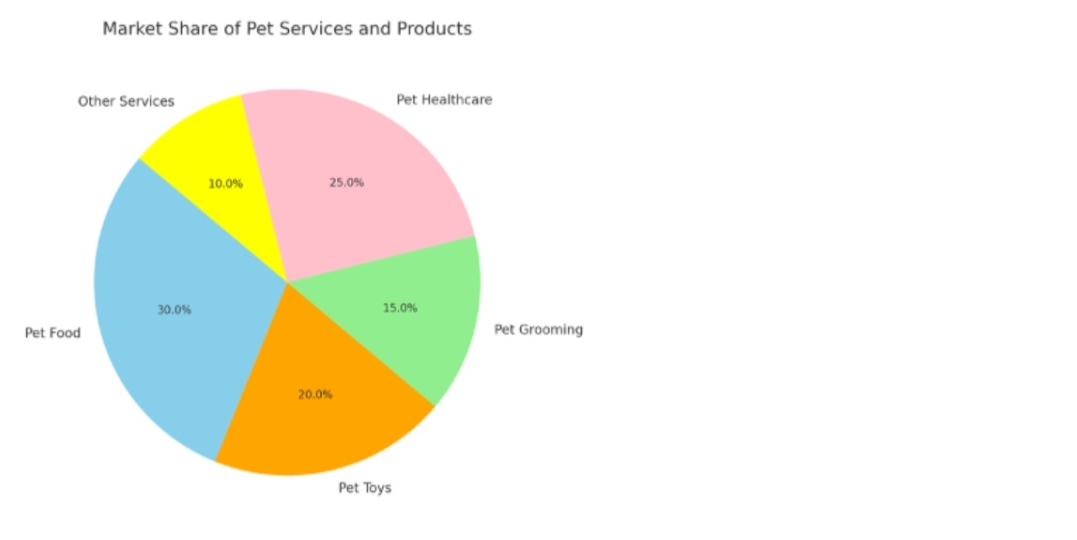
\includegraphics[width=0.86\linewidth]{img/di_pet_services.png}\end{center}
\ptesub{你的作答（语音识别文字稿 ASR Transcript）}
\begin{asrbox}
This pie chart gives information about market share of pet services and products. From the picture we can see in pet grooming the value is 15 percent. In pet toys the proportion is higher, which is 20 percent. The highest number is in pet food, around 30 percent. And the lowest percentage is in other services, just 10 percent. To sum up, the graph tells about pet services and products.
\end{asrbox}
\zh{这张饼图给出的是宠物服务与产品市场份额的信息。从图中可以看到，宠物美容的占比是 15\%；宠物玩具的比例更高，为 20\%；最高的是宠物食品，约 30\%；最低的是其它服务，只有 10\%。总的来说，这张图讲的是宠物服务与产品。}
{\footnotesize\color{gray}（注：作答漏提了 Pet Healthcare 25\% 这一类别，原图饼图共 5 类：Pet Healthcare 25\%、Pet Grooming 15\%、Pet Toys 20\%、Pet Food 30\%、Other Services 10\%。）}
\smallskip
\textbf{总分：}\ {\color{cAccent}\bfseries 10 / 90}\quad{\footnotesize\color{gray}（DI CN V4.0；录音 0:35，用时 01:01）}
\end{qblock}

% ---------------- Q2 ----------------
\begin{qblock}{DI\,2\quad DI \#1186\ \ Estate Sales}{描述图 · 总分 \textcolor{cAccent}{\bfseries 10 / 90}}
\ptesub{配图 Image（柱状图 Bar Chart）}
\begin{center}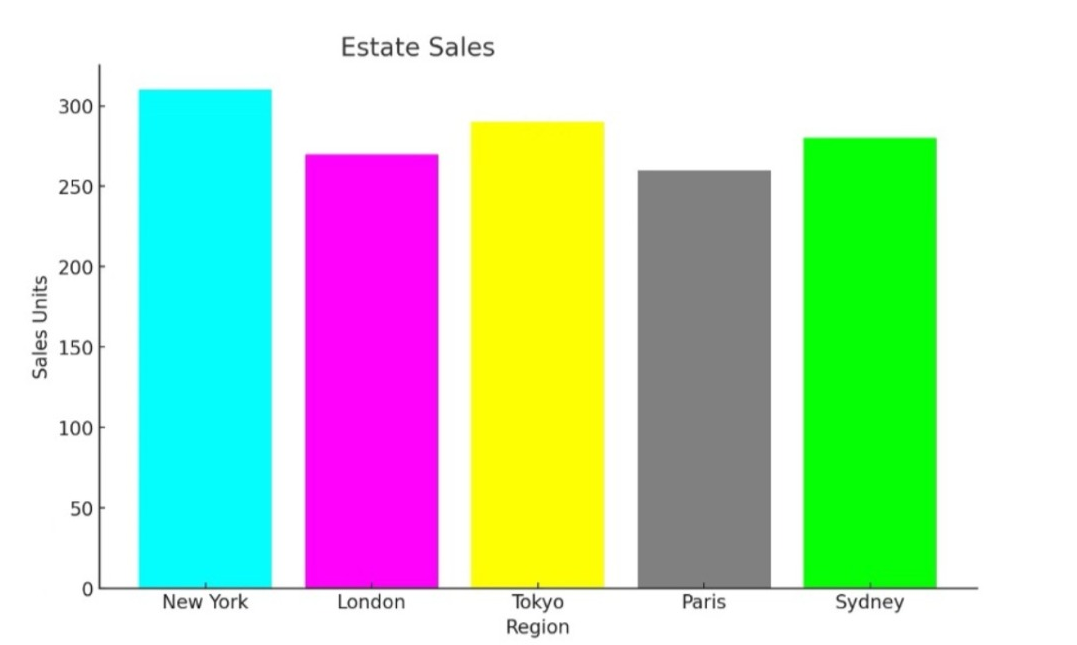
\includegraphics[width=0.86\linewidth]{img/di_estate_sales.png}\end{center}
\ptesub{你的作答（语音识别文字稿 ASR Transcript）}
\begin{asrbox}
This bar chart gives information about estate sales. From the picture we can see in London the value is 260. In Tokyo the number is higher, which is 275. The highest one is in New York, around 310. And the lowest point is in Paris, just 250. To sum up, the graph tells about estate sales.
\end{asrbox}
\zh{这张柱状图给出的是房产销售情况的信息。从图中可以看到，伦敦的数值是 260；东京更高，为 275；最高的是纽约，约 310；最低的是巴黎，只有 250。总的来说，这张图讲的是房产销售情况。}
{\footnotesize\color{gray}（注：作答漏提了 Sydney 这一城市；口述的数值与图中读数略有出入（图中约为 New York 310 / London 270 / Tokyo 290 / Paris 260 / Sydney 280），以图为准。）}
\smallskip
\textbf{总分：}\ {\color{cAccent}\bfseries 10 / 90}\quad{\footnotesize\color{gray}（DI CN V4.0；录音 0:28，用时 00:54）}
\end{qblock}

% ---------------- Q3 ----------------
\begin{qblock}{DI\,3\quad DI \#1148\ \ Electricity Usage}{描述图 · 总分 \textcolor{cAccent}{\bfseries 10 / 90}}
\ptesub{配图 Image（折线图 Line Chart）}
\begin{center}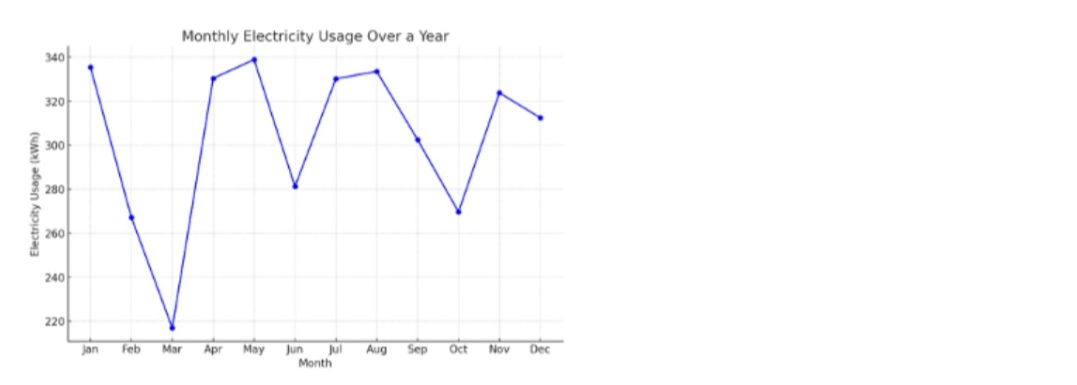
\includegraphics[width=0.86\linewidth]{img/di_electricity_usage.png}\end{center}
\ptesub{你的作答（语音识别文字稿 ASR Transcript）}
\begin{asrbox}
This line chart gives information about monthly electricity usage over a year. From the picture we can see in June the value is 280. In July the number is higher, which is 330. The highest usage is in May, around 340. And the lowest one is in March, just 210. There are many other months, such as August, October and December. To sum up, the graph tells about monthly electricity usage.
\end{asrbox}
\zh{这张折线图给出的是一年中每月用电量的信息。从图中可以看到，六月的数值是 280；七月更高，为 330；最高的是五月，约 340；最低的是三月，只有 210；还有其它一些月份，比如八月、十月和十二月。总的来说，这张图讲的是每月用电量。}
\smallskip
\textbf{总分：}\ {\color{cAccent}\bfseries 10 / 90}\quad{\footnotesize\color{gray}（DI CN V4.0；录音 0:35，用时 01:02）}
\end{qblock}

% ---------------- Q4 ----------------
\begin{qblock}{DI\,4\quad DI \#949\ \ Crop Distribution}{描述图 · 总分 \textcolor{cAccent}{\bfseries 10 / 90}}
\ptesub{配图 Image（世界地图 World Map）}
\begin{center}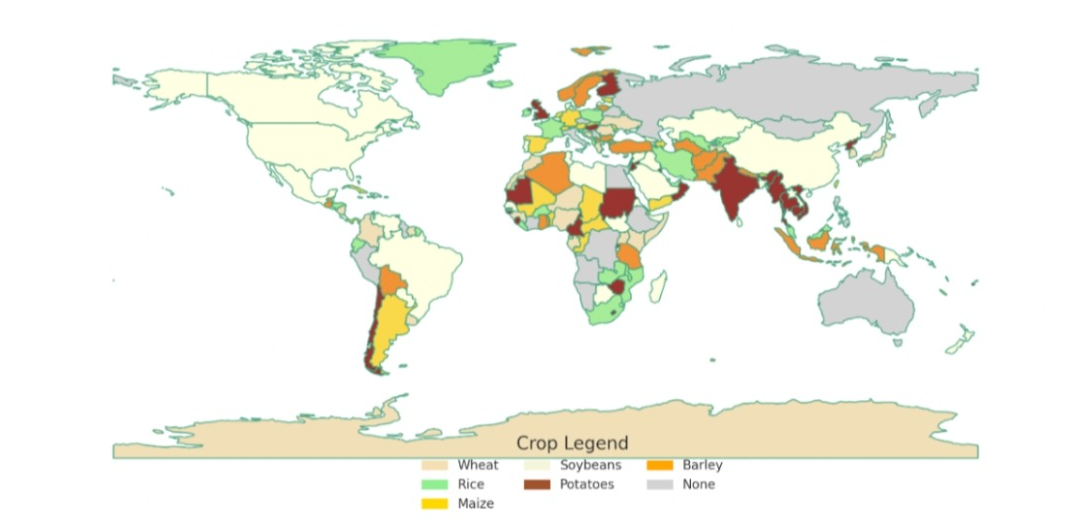
\includegraphics[width=0.9\linewidth]{img/di_crop_distribution.png}\end{center}
\ptesub{你的作答（语音识别文字稿 ASR Transcript）}
\begin{asrbox}
The following graph gives information about the distribution of crops across the world. According to the picture, I can see the geographical locations where crops are predominantly grown. From the picture, in China and North America soybeans are the main agricultural products. Moreover, there are some regions like Russia and Austria with no crop. Lastly, maize is grown in South America. To sum up, the graph tells about distribution of crops.
\end{asrbox}
\zh{这张图给出的是全球作物分布的信息。从图中可以看出作物主要种植的地理位置。从图中看，中国和北美地区大豆是主要农产品；此外，像俄罗斯和奥地利这样的一些地区没有作物；最后，南美洲种植玉米。总的来说，这张图讲的是作物分布情况。}
{\footnotesize\color{gray}（注：口述"Austria"应为"Australia"（澳大利亚，图中该区域标为 None）；图例另有 Wheat / Rice / Barley / Potatoes 类别，作答未逐一提及。）}
\smallskip
\textbf{总分：}\ {\color{cAccent}\bfseries 10 / 90}\quad{\footnotesize\color{gray}（DI CN V4.0；录音 0:39，用时 01:05）}
\end{qblock}

% ---------------- Q5 ----------------
\begin{qblock}{DI\,5\quad DI \#1160\ \ Riverside Town}{描述图 · 总分 \textcolor{cAccent}{\bfseries 10 / 90}}
\ptesub{配图 Image（照片 Photo）}
\begin{center}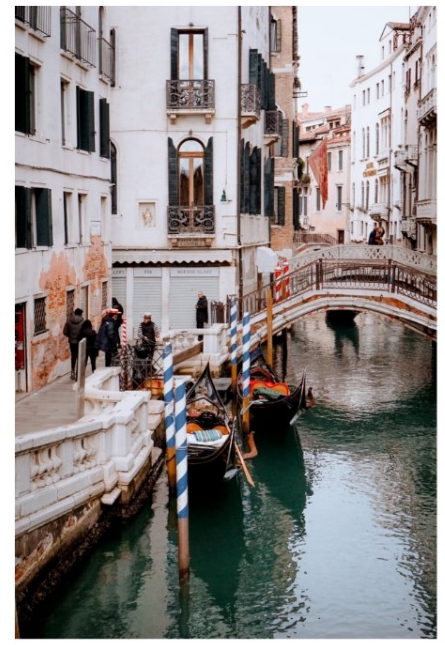
\includegraphics[width=0.55\linewidth]{img/di_riverside_town.png}\end{center}
\ptesub{你的作答（语音识别文字稿 ASR Transcript）}
\begin{asrbox}
The picture gives information about a riverside town. There is a small river in the picture, with an arch bridge over the river. From the picture we can see some small boat in the river, two of which are moored to the bank, one of which is sailing across the bridge. Some tourists are on the bank, seeming to be interested by the boats. On the both banks, a lot of four-storyed buildings are very close to the river. To sum up, the graph tells about a riverside town.
\end{asrbox}
\zh{这张图给出的是一个河边小镇的信息。图中有一条小河，河上有一座拱桥。从图中可以看到河里有几只小船，其中两只停靠在岸边，一只正驶过桥下。岸边有些游客，似乎对这些船很感兴趣。两岸有许多四层楼高的建筑，紧邻河边。总的来说，这张图讲的是一个河边小镇。}
\smallskip
\textbf{总分：}\ {\color{cAccent}\bfseries 10 / 90}\quad{\footnotesize\color{gray}（DI CN V4.0；录音 0:15，用时 00:41）}
\end{qblock}

\end{document}
